\documentclass[11pt,twoside]{article}
\usepackage[utf8]{inputenc}
\usepackage[T1]{fontenc}

% Page margins, header and footer positions
\usepackage{geometry}
\geometry{
 a4paper,
 total={210mm,297mm},
 left=25mm,
 right=25mm,
 top=30mm,
 bottom=25mm,
 headsep=7mm
}

\interfootnotelinepenalty=10000

% To display filling dots in the TOC for all entries
\usepackage[titles]{tocloft}
\renewcommand{\cftsecleader}{\cftdotfill{\cftdotsep}}

% Define new header and footer style
\usepackage{fancyhdr}

\pagestyle{fancy}
\fancyhf{}
\lhead{\color{Gray}{\small{Students\&Companies:RASD}}}
\rhead{\color{Gray}{\small{Riccardo Bonfanti, Jie Chen}}}
\lfoot{\textcolor{Gray}{\small{Copyright © 2024, Riccardo Bonfanti, Jie Chen  – All rights reserved}}}
\rfoot{\textcolor{Gray}{\thepage}}
\renewcommand{\headrulewidth}{0pt}

% PACKAGES
\usepackage{wasysym}
\usepackage{pifont}

\newcommand{\supported}{\ding{52}\xspace}
\newcommand{\unsupported}{\ding{55}\xspace}
\newcommand{\partsupported}{\textcolor{black!40}{\ding{52}}\xspace}
\newcommand{\lowsupported}{\textcolor{black!20}{\ding{52}}\xspace}
\newcommand{\unknowsupported}{\textbf{?}\xspace}

% Font: Times
\usepackage{times}
% Change monospaced font
\renewcommand{\ttdefault}{lmtt}

% Tables
\usepackage{tabu}
\usepackage{tabularx}
\usepackage{ltablex}
\usepackage{longtable}
\usepackage{float}

% Landscape mode
\usepackage{pdflscape}
\usepackage{rotating}
\usepackage{caption}

% Make landscape mode be sensitive to even and odd pages
\def\myrotate{\ifodd\c@page\else-\fi 90}
\makeatletter
\global\let\orig@begin@landscape=\landscape%
\global\let\orig@end@landscape=\endlandscape%
\gdef\@true{1}
\gdef\@false{0}
\gdef\landscape{%
    \global\let\within@landscape=\@true%
    \orig@begin@landscape%
}%
\gdef\endlandscape{%
    \orig@end@landscape%
    \global\let\within@landscape=\@false%
}%
\@ifpackageloaded{pdflscape}{%
    \gdef\pdf@landscape@rotate{\PLS@Rotate}%
}{
    \gdef\pdf@landscape@rotate#1{}%
}
\let\latex@outputpage\@outputpage
\def\@outputpage{
    \ifx\within@landscape\@true%
        \if@twoside%
            \ifodd\c@page%
                \gdef\LS@rot{\setbox\@outputbox\vbox{%
                    \pdf@landscape@rotate{-90}%
                    \hbox{\rotatebox{90}{\hbox{\rotatebox{180}{\box\@outputbox}}}}}%
                }%
            \else%
                \gdef\LS@rot{\setbox\@outputbox\vbox{%
                    \pdf@landscape@rotate{+90}%
                    \hbox{\rotatebox{90}{\hbox{\rotatebox{0}{\box\@outputbox}}}}}%
                }%
            \fi%
        \else%
            \gdef\LS@rot{\setbox\@outputbox\vbox{%
                \pdf@landscape@rotate{+90}%
                \hbox{\rotatebox{90}{\hbox{\rotatebox{0}{\box\@outputbox}}}}}%
            }%
        \fi%
    \fi%
    \latex@outputpage%
}
\makeatother

% Graphics
\usepackage{graphicx}
\usepackage[dvipsnames, table]{xcolor}

% Other
\usepackage{ifthen}
\usepackage{xspace}
\usepackage{enumitem}
\usepackage{amssymb}
\usepackage[pdftex, colorlinks]{hyperref}
\newcommand{\comment}[1]{{\color{Red}$\blacktriangleright$ Comment: #1 $\blacktriangleleft$}}

% Some utilities
\usepackage{soul}
\usepackage{tikz}

\usetikzlibrary{calc}
\usetikzlibrary{decorations.pathmorphing}


\makeatletter

\newcommand{\defhighlighter}[3][]{%
  \tikzset{every highlighter/.style={color=#2, fill opacity=#3, #1}}%
}

\defhighlighter{yellow}{.5}

\newcommand{\highlight@DoHighlight}{
  \fill [ decoration = {random steps, amplitude=1pt, segment length=15pt}
        , outer sep = -15pt, inner sep = 0pt, decorate
       , every highlighter, this highlighter ]
        ($(begin highlight)+(0,8pt)$) rectangle ($(end highlight)+(0,-3pt)$) ;
}

\newcommand{\highlight@BeginHighlight}{
  \coordinate (begin highlight) at (0,0) ;
}

\newcommand{\highlight@EndHighlight}{
  \coordinate (end highlight) at (0,0) ;
}

\newdimen\highlight@previous
\newdimen\highlight@current

\DeclareRobustCommand*\highlight[1][]{%
  \tikzset{this highlighter/.style={#1}}%
  \SOUL@setup
  %
  \def\SOUL@preamble{%
    \begin{tikzpicture}[overlay, remember picture]
      \highlight@BeginHighlight
      \highlight@EndHighlight
    \end{tikzpicture}%
  }%
  %
  \def\SOUL@postamble{%
    \begin{tikzpicture}[overlay, remember picture]
      \highlight@EndHighlight
      \highlight@DoHighlight
    \end{tikzpicture}%
  }%
  %
  \def\SOUL@everyhyphen{%
    \discretionary{%
      \SOUL@setkern\SOUL@hyphkern
      \SOUL@sethyphenchar
      \tikz[overlay, remember picture] \highlight@EndHighlight ;%
    }{%
    }{%
      \SOUL@setkern\SOUL@charkern
    }%
  }%
  %
  \def\SOUL@everyexhyphen##1{%
    \SOUL@setkern\SOUL@hyphkern
    \hbox{##1}%
    \discretionary{%
      \tikz[overlay, remember picture] \highlight@EndHighlight ;%
    }{%
    }{%
      \SOUL@setkern\SOUL@charkern
    }%
  }%
  %
  \def\SOUL@everysyllable{%
    \begin{tikzpicture}[overlay, remember picture]
      \path let \p0 = (begin highlight), \p1 = (0,0) in \pgfextra
        \global\highlight@previous=\y0
        \global\highlight@current =\y1
      \endpgfextra (0,0) ;
      \ifdim\highlight@current < \highlight@previous
        \highlight@DoHighlight
        \highlight@BeginHighlight
      \fi
    \end{tikzpicture}%
    \the\SOUL@syllable
    \tikz[overlay, remember picture] \highlight@EndHighlight ;%
  }%
  \SOUL@
}

\makeatother



\begin{document}

% TITLE PAGE
\begin{titlepage}
% LOGO
\begin{table}[t!]
\centering
\begin{tabu} to \textwidth { X[1.3,r,p] X[1.7,l,p] }
\textcolor{Blue}{\textbf{\small{Students\&Compagnies}}} & 
\includegraphics[scale=0.5]{Images/PolimiLogo} \\
\end{tabu}
\begin{tabu} to \textwidth { X[1.3,r,p] X[1.7,l,p] }
    \textcolor{Blue}{\textbf{\small{Riccardo Bonfanti | Jie Chen}}} &\\
    \end{tabu}
\end{table}~\\ [7cm]

% TITLE 
\begin{flushleft}
{\textcolor{Blue}{\textbf{\Huge{Requirement Analysis and Specification
        Document}}}} \\ [1cm]
\end{flushleft}
\end{titlepage}

% Define deliverable specific info
\begin{table}[h!]
\begin{tabu} to \textwidth { X[0.3,r,p] X[0.7,l,p] }
\hline
\textbf{Deliverable:} & RASD\\
\textbf{Title:} & Requirement Analysis and Verification Document \\
\textbf{Authors:} & Riccardo Bonfanti, Jie Chen \\
\textbf{Version:} & 1.0 \\ 
\textbf{Date:} & 22-December-2024 \\
\textbf{Download page:} & https://github.com/JieCver1/BonfantiChen \\
\textbf{Copyright:} & Copyright © 2024, Riccardo Bonfanti, Jie Chen – All rights reserved \\
\hline
\end{tabu}
\end{table}

\setcounter{page}{2}

\newpage
%\addcontentsline{toc}{section}{Table of Contents}

\tableofcontents

%\newpage
%\addcontentsline{toc}{section}{List of Figures}
%\listoffigures
%\addcontentsline{toc}{section}{List of Tables}
%\listoftables

\clearpage
{\color{Blue}{\section{Introduction}}}
\label{sect:introduction}
% chktex-file 44
\renewcommand{\thesection}{\Alph{section}}
\section{Purposes and Goals}\label{sec:purposeandgoals}
\subsection{Purpose}\label{subsec:purpose}
Internships provide students with a valuable opportunity to apply their skills in real job environments while enabling companies to connect with 
fresh talent. However, the process of finding and securing internships can be challenging for both parties.

Students\&Companies (S\&C) is a platform designed to facilitate this connection throughout the internship process. It allows 
students to match their preferences with available opportunities, ensuring internships align with their experiences and skills. 
Companies can specify project requirements to attract suitable candidates.

The platform supports both students and companies in two phases: recommendation and selection. It utilizes keyword searches 
and statistical analyses to evaluate internship and student data, ensuring a match that meets the needs of both parties. 
Students can search for internships and receive notifications about appealing opportunities, while companies can publish offers and get 
alerts when student CVs match their criteria. Once mutual interest is established, the selection phase begins, where the platform assists 
with interviews and finalizes the process. It also monitors the internship journey, providing the possibility to exchange feedback and 
enabling direct communication to address any questions. Additionally, the universities of the students can oversee the process to ensure 
that everything is going smoothly.

\subsection{Goals}\label{subsec:goals}
[G1] All unregistered Users must be able to create an account on the platform using their specific email address and log in to the platform.

[G2] Students must be able to upload their CVs on the platform.

[G3] Students must be able to search for available internship offers on the platform.

[G4] Companies must be able to publish internship offers on the platform.

[G5] Users must receive notifications about relevant events.

[G6] Students and Companies must receive recommendations based on statistical analyses.

[G7] Students must be able to proactively apply for internships, before the submission deadline.

[G8] Companies must be able to set up the interview process.

[G9] During the interview process, students must be able to respond to the company's questions through questionnaires.

[G10] At the end of the interview process, companies must be able to collect the students' responses.

[G11] Companies must be able to send the results of the interviews to the students.

[G12] Students must be able to accept or reject the internship offer after receiving the interview results.

[G13] Students and companies must be able to write feedback regarding their internship experiences.

[G14] Students and companies must be able to communicate with each other during internship process.

[G15] Universities must be able to monitor the internship process of their students.


\newpage
\section{Scope}\label{sec:scope}
\subsection{Scope}\label{subsec:scope}
Students\&Companies (S\&C) aims to provide the best matching service between students and companies for internships. The platform will be available
to students, companies, and universities.

If it is their first time using the platform, Students looking for internships can create an account using their educational institution's email and 
select their university from a list of the ones that collaborate with the platform. 
After creating an account, they need to fill out their profiles to describe their skills, experiences, and preferences. To complete
their profiles, they must also upload their CVs.
Otherwise they can log in to the platform using their credentials.

The universities associated with the students through their educational emails will be notified about the students' registration on the platform. 
The system will then add the registered students to the university’s list, allowing the universities to monitor their internship activities.

Companies wishing to announce internship opportunities can create an account on the platform, if they do not already have one. They need to
provide the necessary information for the internship announcement such as the job description, requirements, and the number of interns needed etc. 
Companies can also specify the skills they are looking for in students.

The platform will extract key information from the students' profiles and the companies' internship announcements, along with historical feedback and 
information collected from previous internships, to recommend the best matches for both parties. Students will receive notifications about 
recommended internships, and companies will be alerted when existing students with matching CVs meet their needs.

Once students apply for the offers they are interested in, the companies will receive the applications and can select the students they wish 
to interview. The platform will assist companies in setting up the interview process and will allow them to record and store students' responses 
using the platform. Students will be able to respond to companies' questions through the tools or channels provided.

At the end of the interviews, companies can send the results to the students. Upon receiving the results, students can decide whether to accept 
or reject the offer, and the companies will be notified of their decisions. If a student accepts the offer and starts the internship, the platform 
will update the internship activities about that student at their universities. Students and companies can use the channels provided by the platform to
communicate with each other during the internship, and also they can provide feedback and complains regarding their experiences in dedicated section
which can be monitored by the students' universities. 

\subsection{Phenomena}
Referring to the Jackson-Zave distinction between the world and the machine in the context of the S\&C platform, the following phenomena are 
identified, specifying which parts are controlled by the machine and which parts are controlled by the world, shown in table~\ref{table:phenomena}.

\begin{table}[H]
    \caption*{\textbf{Phenomena based on the Jackson-Zave model}}
    \centering 
    \begin{tabular}{|c|p{24em}|c|c|}
    \hline
    \rowcolor{bluepoli!40} % comment this line to remove the color
    \small\textbf{Code} & \small\textbf{Phenomenon} & \small\textbf{Shared} & \small\textbf{Control} \T\B \\
    \hline
    \small\textbf{P1} &\small \textbf{User registration} & Yes & World \T\B \\
    \small\textbf{P2} &\small \textbf{User login} & Yes & World \T\B\\
    \small\textbf{P3} &\small \textbf{Check username and password} & No & Machine \T\B\\
    \small\textbf{P4} &\small \textbf{Student creates CV using text editor} & No & World  \T\B \\
    \small\textbf{P5} &\small \textbf{Student uploads CV in profile} & Yes & World  \T\B \\
    \small\textbf{P6} &\small \textbf{Student updates profile information} & Yes & World  \T\B \\
    \small\textbf{P7} &\small \textbf{Student searches available internships} & Yes & World \T\B\\
    \small\textbf{P8} &\small \textbf{Company publishes internship offers} & Yes & World \T\B \\
    \small\textbf{P9} &\small \textbf{Platform notifies users that a deadline has expired} & Yes & Machine \B\\
    \small\textbf{P10} &\small \textbf{Platform suggests recommendations} & Yes & Machine \T\B \\
    \small\textbf{P11} &\small \textbf{Platform adds student to university's list} & No & Machine \T\B \\
    \small\textbf{P12} &\small \textbf{A student submits an application for an internship} & Yes & World \B\\
    \small\textbf{P13} &\small \textbf{Company selects candidates to interview} & Yes & World \T\B\\
    \small\textbf{P14} &\small \textbf{Student participates to the interview} & Yes & World \T\B \\
    \small\textbf{P15} &\small \textbf{Company sends interview results} & Yes & World \B\\
    \small\textbf{P16} &\small \textbf{Student accepts or rejects the internship} & Yes & World \T\B \\
    \small\textbf{P17} &\small \textbf{ST and CO write feedback on the internship} & Yes & World \T\B\\
    \small\textbf{P18} &\small \textbf{ST and CO view feedback on the internship} & Yes & World \B\\
    \small\textbf{P19} &\small \textbf{Student views the offers' description} & Yes & World \T\B \\
    \small\textbf{P20} &\small \textbf{Company views the students' profile} & Yes & World \T\B\\
    \small\textbf{P21} &\small \textbf{University views the list of its students} & Yes & World \B\\
    \small\textbf{P22} &\small \textbf{University tracks the internship process} & Yes & World \T\B\\
    \hline
    \end{tabular}
    \\[10pt]
    \caption{Phenomena in the S\&C context}\label{table:phenomena}
\end{table}

\section{Definitions, Acronyms, Abbreviations}\label{sec:definitions}
\subsection{Definitions}\label{subsec:definitions}
\begin{itemize}
    \item \textbf{Student:} A person who is looking for internships.
    \item \textbf{Company:} An organization which wants to announce internship opportunities to students.
    \item \textbf{University:} An educational institution that is related to students and their internships.
    \item \textbf{User:} A generic term for students, companies, and universities who use the platform.
    \item \textbf{Candidate:} A term for students whose applications are selected and that will take part in the interview process.
    \item \textbf{Internship:} A opportunity offered by companies to students to gain practical experience in a real job environment.
    \item \textbf{CV:} Curriculum Vitae, a document that contains all necessary information about students to be able to apply for internships.
    \item \textbf{Recommendation:} A suggestion made by the platform to students and companies based on statistical analyses and keyword searches.
    \item \textbf{Selection:} The process of choosing students and companies to process the interview.
    \item \textbf{Feedback:} Helpful information written by students and companies about their internship experiences to improve a performance 
    of the two parties.
    \item \textbf{Notification:} A message sent by the platform to inform students and companies about important events, such as new internship 
    offers, matching CVs, interview results etc.
    \item \textbf{Interview:} A meeting between students and companies to decide an assignment of the internship offer.
    \item \textbf{Platform:} The Students\&Companies (S\&C) system that provides the services to students, companies, and universities about
    internships.
    \item \textbf{Keyword:} A significant word or tag used to describe content, such as the skills, experiences, and preferences of students and 
    companies.
    \item \textbf{Comment:} The text that is written by students and companies to provide feedback or complaints about their internship experiences.
    \item \textbf{Complain:} A text that expresses dissatisfaction, issues, or annoyance about the internship experiences.
\end{itemize}

\subsection{Acronyms}\label{subsec:acronyms}
\begin{itemize}
    \item \textbf{S\&C:} Students\&Companies
    \item \textbf{CV:} Curriculum Vitae
    \item \textbf{UI:} User Interface
    \item \textbf{UX:} User Experience
    \item \textbf{API:} Application Programming Interface
    \item \textbf{HTTP:} Hypertext Transfer Protocol
    \item \textbf{HTTPS:} Hypertext Transfer Protocol Secure
    \item \textbf{TLS:} Transport Layer Security
    \item \textbf{REST:} Representational State Transfer

\end{itemize}

\subsection{Abbreviations}\label{subsec:abbreviations}
\begin{itemize}
    \item \textbf{[Gn]:} Used to number the goals, where Gn is the n-th goal.
    \item \textbf{[Pn]:} Used to number the phenomena, where Pn is the n-th phenomenon.
    \item \textbf{[Rn]:} Used to number the requirements, where Rn is the n-th requirement.
    \item \textbf{[An]:} Used to number the domain assumptions, where An is the n-th assumption.
    \item \textbf{CO:} Company
    \item \textbf{ST:} Student
    \item \textbf{UNI:} University
\end{itemize}

\section{Revision History}\label{sec:revisionhistory}
%%TODO

\section{Reference Documents}\label{sec:reference}
\begin{itemize}
    \item `` The World and the Machine: A model for the functional architecture '' by Michael Jackson and Pamela Zave.
    \item Assignment RDD AY 2024–2025.
\end{itemize}

\section{Document Structure}\label{sec:structure}
This document is structured as follows:
\begin{itemize}
    \item \textbf{Section 1: Introduction} 
    \\It contains the purpose, goals, scope, and phenomena identified in the context of the S\&C project, 
    including the specification of definitions, acronyms, and abbreviations of the terms used in this document. In addition, it notes the revision 
    history for updates to the document and the reference documents that were used during the development of this document.
    \item \textbf{Section 2: Overall Description}
    \\ In this section, the general view of the S\&C project is presented, including the product perspective, functions, characteristics, 
    constraints, assumptions, and dependencies. Through the use of UML diagrams, the statecharts, and the scenarios to explain the project's 
    functionalities.
    \item \textbf{Section 3: Specific Requirements}
    \\ A detailed description of the requirements of the project will be provided in this section. Using the various point of views, the external   
    interface requirements, functional requirements, performance requirements, design constraints, software system attributes, and other 
    requirements. In particular to easier understanding, the use cases, sequence diagrams, mapping tables and simple drafts of the user interface 
    will be presented.
    \item \textbf{Section 4: Formal Analysis}
    \\ Using the Alloy language to model the project and to verify the logical consistency of the model. It will also be used to check the
    correctness of the requirements and to present the main features guaranteed by the platform. Also, a part of the scenarios will be presented 
    by predicates using show and run commands.
    \item \textbf{Section 5: Effort Spent}
    The time spent by each group member on each task will be registered in this section. It will be used to present the effort dedicated 
    by each member and to present the progress of the development of the project.
    \item \textbf{Section 6: References}
    \\ The other references that not include in the reference documents will be added in this section.
\end{itemize}

\clearpage
{\color{Blue}{\section{Overall Description}}}
\label{sect:overview}
\renewcommand{\thesection}{\Alph{section}}
\section{Product perspective}\label{sec:product_perspective}
\subsection{Scenarios}\label{subsec:scenarios}
\subsubsection{Scenario 1: Mr.Spongebob registers on the platform}\label{subsubsec:scenario_1}
Mr.Spongebob, a final-year student at the University of Bikini Bottom, is looking for an internship to practice the knowledge he's gained. 
To do so, he asks advice from Professor Puff, who suggests using the Students\&Companies platform to search for internship opportunities.
Following her advice, Mr.Spongebob registers as a student on the platform, selecting the University of Bikini Bottom from the list of 
universities and verifying his student status with his educational email and password. Then, he fills in all the required personal information,
including his name, date of birth, and other details. He also inserts keywords to describe his skills and the job fields he might be interested 
in. Finally, after uploading his CV, which contains all the necessary information and details, Mr.Spongebob completes his registration and 
can begin searching for internships. Meanwhile, Professor Puff, who oversees internship activities using the official account of the University of 
Bikini Bottom, is notified of Mr.Spongebob's registration.

\subsubsection{Scenario 2: Mr.Krabs publishes an internship offer}\label{subsubsec:scenario_2}
Due to the rapid evolution of Technology, Mr.Krabs decides to collaborate with his competitor Mr.Plankton, on a new project. They 
plan to develop a ``Hamburger super secret formula detector'' that can detect what the customer likes by looking at his facial expressions, in 
order to to create the perfect personalized hamburger! To achieve this, they need to hire students specializing in Computer Vision, Deep Learning and
AI to study the visual data. So Mr.Krabs logs into the Students\&Companies platform using the official company account
and navigates to the ``Publish Internship'' section to create a new announcement. He fills in all the required information: 
the title, location, role, application deadline, number of positions, duration, employment type, description, and required skills.
After that, Mr.Krabs published the internship offer, which can be seen in the ``Available Internships'' section. Immediately after 
the publication, he receives a notification of recommended student profiles that may match the offer requirements.
\begin{quote}
    \begin{center}
       \textbf{\textquotedbl Computer Vision and AI Intern\textquotedbl}
    \end{center}
    
    \textit{Location:} Krusty Krab Technology Lab, Bikini Bottom \\
    \textit{Role:} Intern \\
    \textit{Application Deadline:} 25th December 2024 \\
    \textit{Number of Positions:} 2 \\
    \textit{Duration:} 6 months \\
    \textit{Employment Type:} Full-time \\
    \textit{Description:} We are looking for students who can contribute to the development of the Hamburger super secret formula detector by developing 
    algorithms that collect and analyze visual data. A love for hamburgers is essential!\\
    \textit{Required Skills:} Computer Vision, AI, Python, Deep Learning
\end{quote}

\subsubsection{Scenario 3: Mr.Patrick searches internship}\label{subsubsec:scenario_3}
Mr.Patrick is very worried because he is in the last semester of his master's degree, so he has to find an internship or he won't be able to graduate in Food Engineering.
He remembers he has an account on the Students\&Companies platform, which he used to find an internship at the beginning of his studies, so he decides 
to take another look at the platform. He logs in and updates his profile and CV, adding the new skills he has acquired during his master’s degree.
He navigates to the search bar and types ``Hamburger'' to look for internships related to hamburger studies. When he doesn’t find anything that 
interests him, he scrolls through the recommended internships list. Finally, he finds Mr.Krabs' posting and becomes very interested in the 
project, so he applies for the internship and waits for the company's response. After applying, he can check the status of his application in 
the ``Your Applications'' section.

\subsubsection{Scenario 4: Krusty Krab Technology Lab Interview}\label{subsubsec:scenario_4}
After the application deadline, Mr.Krabs and Mr.Plankton review all the applications received for the intern position. They select the
candidates by reviewing their profiles and CVs, and then send them an invitation for an interview. For the first round of interviews, Mr.Plankton
decides to formulate a set of short questions to know more about the candidates' skills and experiences. The candidate will be able to respond to 
these questions through a form inside the platform. In said form Mr.Plankton also includes the date, time and location of the interview and the 
necessary information to better prepare the candidates. After sending the invitations, the candidates selected for the interview receive a notification 
from the platform, who is not selected will receive a notification of rejection. At the end of the interview, Mr.Plankton evaluates the candidates 
and discusses with Mr.Krabs to decide who to hire. Finally, they send an offer to the best candidates and wait for their acceptance to start the internship.

\subsubsection{Scenario 5: Ms.Sandy starts her internship}\label{subsubsec:scenario_5}
Ms.Sandy is very passionate about space and is thrilled to have been selected for an internship at the Underwater Space Agency. She receives 
and accepts an offer from the company. At the same time, the Bikini Bottom University of Aerospace's professor Manta received the notification
about the new activity started by Sandy. However, she is a bit anxious, so she logs into the platform and navigates to the ``Internship'' 
section to find her assigned mentor's profile. She starts a chat with him to ask some questions about how she should prepare in the coming days
and for any advice he can give her to have a good start in the internship.

\subsubsection{Scenario 6: Mr.Squidward leaves his feedback}\label{subsubsec:scenario_6}
At the end of his internship at the ``Krusty Krab Technology Lab'' as a data science intern, Mr.Squidward is surprised by the experience 
he has gained, even though he has several complaints about the heavy workload. He decides to leave a warm message for Mr.Krabs and Mr.Plankton 
to thank them for the opportunity. After that, he navigates to the ``Internship'' section to add a review of his internship experience and rate 
the company. It is also the section where he can check the suggestions left by his mentors regarding his internship, which is only visible to the 
company and the university.

\subsubsection{Scenario 7: Track the internship activities}\label{subsubsec:scenario_7}
As the internship period progresses, Professor Puff is responsible for overseeing the students' activities at the University of Bikini Bottom. 
She is curious to know how the students are doing in their internships, particularly Mr.SpongeBob, who is using the platform for the first time. 
She logs into the platform with the university credentials and looks at the list of students, searching for SpongeBob's name. She finds, 
in his active internship section, that he has been selected for an internship at the ``Krusty Krab Technology Lab''. By reading the feedback 
left by the company throughout the different stages of the internship, she is very glad to see that SpongeBob is doing well in the field he is 
passionate about!


\subsection{Domain-level diagram}\label{subsec:domain_level_diagram}
%TODO add domain-level diagram

\subsection{Statecharts}\label{subsec:statecharts}

\subsubsection{1. Internship recommendation}\label{subsubsec:internship_application}
\begin{figure}[H]
    \centering
    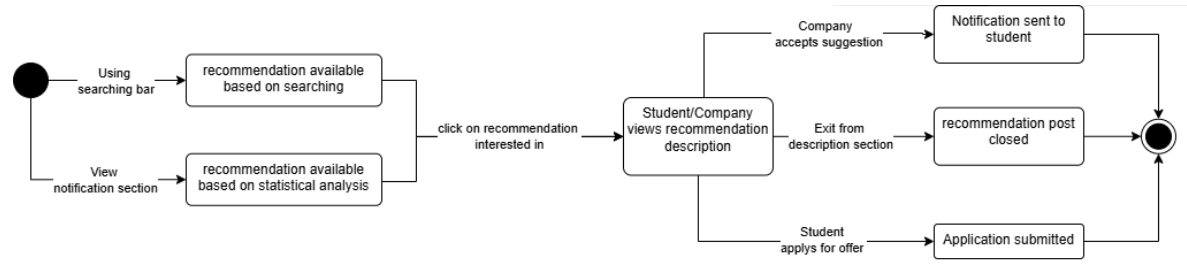
\includegraphics[width=1\textwidth]{Images/Internship_recommendation.png}
    \caption{Statechart diagram for internship recommendation}\label{fig:statechart_internship_recommendation}
\end{figure}
%TODO add description

\subsubsection{2. Selection process for internship}\label{subsubsec:internship_feedback}
\begin{figure}[H]
    \centering
    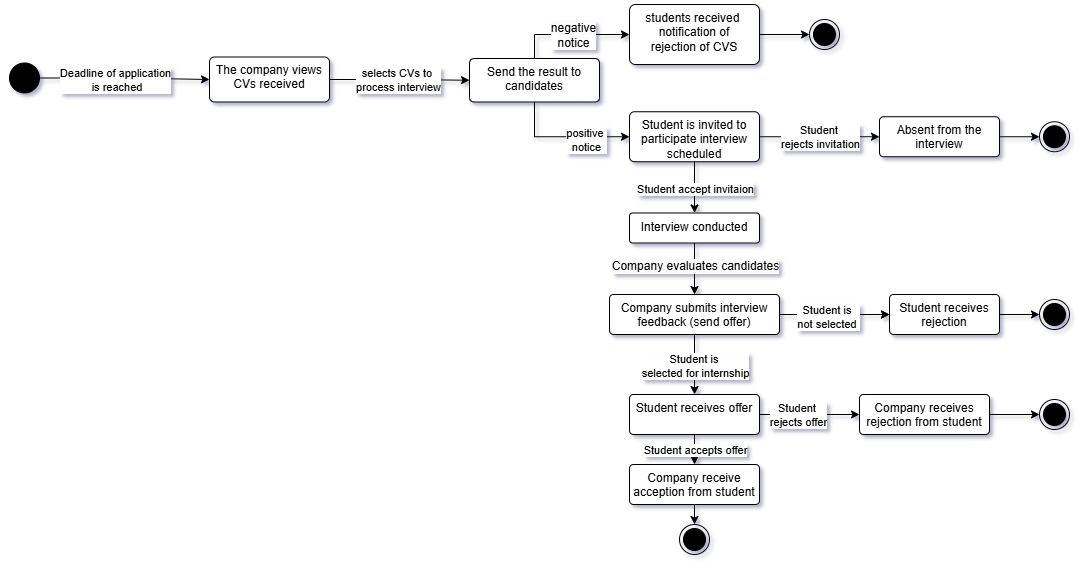
\includegraphics[width=1\textwidth]{Images/Selection_process.png}
    \caption{Statechart diagram for selection process for internship}\label{fig:statechart_selection_process_for_internship}
\end{figure}
%TODO add description

\subsubsection{3. Internship status}\label{subsubsec:monitoring_student_activities}
\begin{figure}[H]
    \centering
    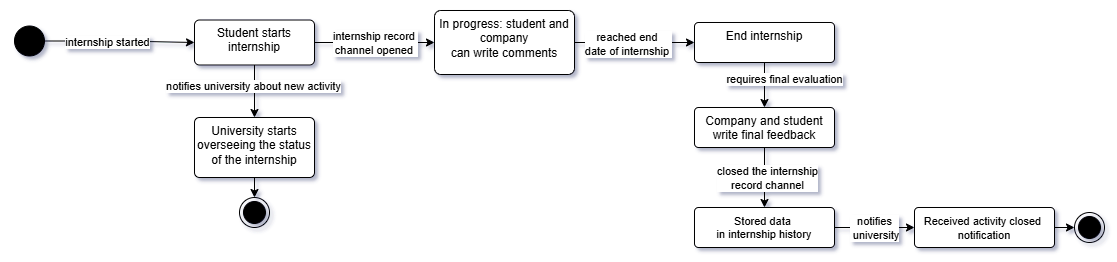
\includegraphics[width=1\textwidth]{Images/Internship_status.png}
    \caption{Statechart diagram for internship status}\label{fig:statechart_internship_status}
\end{figure}
%TODO add description

\section{Product functions}\label{subsec:product_functions}
\begin{itemize}
    \item \textbf{Sign up and login} 
    \item \textbf{Data management system}
    \item \textbf{Search system} 
    \item \textbf{Recommendation system} 
    \item \textbf{Internship application} 
    \item \textbf{Internship Posting}
    \item \textbf{Selection Assistance} 
    \item \textbf{Internship Status Tracking} 
    \item \textbf{Internship Feedback}
    \item \textbf{Monitoring student activities} 
    \item \textbf{Chat system} 
    \item \textbf{Notification system} 
    \item \textbf{Application Acceptance and Rejection} 
\end{itemize}

\section{User characteristics}\label{subsec:user_characteristics}


\section{Domain Assumptions}\label{subsec:domain_assumptions}

\clearpage
{\color{Blue}{\section{Specific Requirements}}}
\label{sect:requirements}
\renewcommand{\thesection}{\Alph{section}}
\section{External Interface Requirements}
\subsection{User Interfaces}
As the users of the platform include students, companies, and universities, the user interface is designed to facilitate interaction with 
the platform and meet their needs. For instance, many students may be unfamiliar with the internship search process and may lack experience
in finding job opportunities, so the user interface should be simple and intuitive to use.

In the following section, the principal Graphical User Interfaces (GUIs) are described within drafts, and this part will be further detailed
using refined mockups in the Design Document
\begin{itemize}
    \item \textbf{Welcome page:} The welcome page is the first page users see when they open the platform. It contains the platform's logo 
    and a brief description of its purpose. On this page, users can log in using their credentials or create an account if they are new
    to Students \& Companies.
    
    \item \textbf{Register Page:} During the registration phase, users will first be asked to select their user type (student, company, or
     university). Based on the selected user type, the corresponding registration form will be displayed, and users will be prompted to 
     provide the necessary information to create an account. In addition to common data such as name, email, and password, users will
     need to provide additional information based on their user type. For example, students and companies will be asked to personalize 
     their profiles by adding details such as their field of interest, skills, a short description of themselves, and more to make their
      profiles more appealing to other users.
    
    \item \textbf{Notification Page:} It will display various types of notifications received from the platform. For example, students will
    see notifications about updates on their application status, companies will receive notifications about new applications, and 
    universities will be notified about new student registrations on the platform.

    \item \textbf{Side Menu:} The side menu is a navigation menu that provides access to the main sections of the platform, depends on the
    user's type. It will be displayed on the left side of the screen, with different sections available. For example, for students, the 
    side menu will include sections such as Search Internships, Dashboard, My Profile, My Applications, Internship History, Chat.

    \item \textbf{Header Bar:} The header bar is displayed at the top of the screen and includes the platform's logo, a menu icon, a chat 
    icon, a notification icon, and the user's profile icon. It remains visible on all pages once the user has logged in.

    \item \textbf{Chat Interface:} The chat interface is accessible from either the side menu or the header bar of the platform. It allows 
    students and companies to communicate with each other in real-time. They can view a list of available chats, send and receive messages, 
    and access their chat history.

    \item \textbf{Profile Page:} This interface is used by user to view and edit their profile data in case of necessary, in particular
    the student can update their CV accessing this page.

    \item \textbf{Search page:} This page contains a search bar and displays the results based on the user's search. For example, a student
    can search for internships, and the platform will return a list of results based on the student's input. 
    
    \item \textbf{Internship evaluation page:} This page is used by both students and companies to evaluate internship performance. Both 
    parties can provide feedback during the internship, and at the end, to complete the evaluation process, they must leave final comments 
    and rate the internship. Students also have the option to leave anonymous reviews about their experience, which can help other students
    make decisions about internships. These reviews will be visible when user visiting the company's profile.

\end{itemize}

Since the platform is designed for three types of users, the specialized interfaces for each user type are described in further detail
below, considering the characteristics of each user.
\begin{itemize}
    \item \textbf{Student Interface:}
    \begin{itemize}
        \item \textbf{Student Dashboard:} This is the home page that appears once the student logs in. On this page, the student gets an 
        overview of all the main functionalities they can access. The dashboard consists of:

        1. Search Bar with Filter Command: Allows the student to search and filter based on specific criteria.
        
        2. Overview of Suggested Internships: Displays job search keywords and internships recommended by the platform's algorithm.
        
        3. My Applications: Provides a quick overview of the status of the student's applications.
        
        4. Internship History: Displays a record of the internships the student has applied for in the past, including the internship they 
        are currently doing if exist.

        \item \textbf{My applications:} The student can track the status of their applications and view the details of the internships 
        they have applied for. Through this interface, the student can also receive information related to the selection process, such 
        as the interview date, the interview result, and the final decision of the company. Additionally, the student can filter their 
        applications based on their status, such as ``waiting''.

        \item \textbf{Internship history:} The student can view the internships they have participated in so far, along with the 
        evaluations related to their experiences. The page also allows the student to access the feedback section, where they can 
        leave comments or notes about a specific internship.

    \end{itemize}
    \item \textbf{Company Interface:} 
    \begin{itemize}
        \item \textbf{Company Dashboard:} It's the home page once the company logs in. On this page, the company gets an overview of 
        all the main functionalities they can access. The dashboard consists of:

        1. Search Bar with Filter Command: Allows the company to search and filter results based on specific criteria.
        
        2. Overview of Student Profiles: Displays student profiles suggested by the platform's matching algorithm for different internship 
        announcements.
        
        3. Internship Announcements: A list of internship announcements the company has published, along with the number of the applications
        received.
        
       \item \textbf{Publish Internship Page:} This is the main functionality of the company interface. On this page, the company can 
       create a new internship announcement and post it on the platform. The company is required to enter the necessary information, 
       following the guidelines provided by the platform.

        \item \textbf{Internship management page:} This page is divided into several sections: one for internship announcements that have 
        been published but are still in the publication phase, one for internships in the selection phase, one for internships currently 
        in progress, and one for closed internships. From this interface, the company can manage internships of all phases.
    \end{itemize}

    \item \textbf{University Interface:} 
    \begin{itemize}
        \item \textbf{University Dashboard:} The university dashboard displays a list of students and their associated activities. 
        The university can view the list of students registered on the platform and select a student to see detailed information about 
        their profile, activities, and internships they are currently doing or have completed in the past.
    \end{itemize}
\end{itemize}


\subsection{Hardware Interfaces}
Students\&Companies is a web-based platform, so it can be accessed from any device with an internet connection. The platform is
compatible with all modern web browsers. It is designed to be responsive and work on different screen sizes, including desktops, 
laptops, tablets, and smartphones. \\
The system will be hosted on multiple server that meet the requirements for web hosting. They will be responsible for the platform's 
backend processes, including the reccomendation algorithm, the data collection and the statistical analyses.


\subsection{Software Interfaces}
The system will interact with an emailing system to confirm the registration of new users. \\
It will also integrate various APIs to provide additional functionalities, for instance an API for implementing statistical analyses 
based on collected data that will be used to improve the recommendation algorithm. Another example would be an API to interact with
the database in order to store and retrieve information.


\subsection{Communication Interfaces}
The system will use HTTPS to ensure secure communication between the client and the server. The platform will also use WebSockets to
enable real-time communication between users, such as chat and notifications functionalities. Since the platform is designed to be a 
RESTful web application, it will use JSON as the data interchange format between the client and the server. \\
To interact with the mailing system, the platform will use SMTP protocol.


\section{Functional Requirements}
\subsection{Functional Requirement}
\subsection{Requirement Mapping}
\subsection{Use Case Diagram}
\subsection{Traceability Matrix}


\section{Performance Requirements}
\begin{itemize}
    \item \textbf{Concurrent access of users and resource utilization:} A platform like Students\&Companies is expected to have a large
    number of users, so it must be able to handle multiple requests simultaneously. By searching online for platforms that offer similar
    services we have found that a good estimate for the number of concurrent users that the platform should be able to manage is roughly
    a few thousands, peaking at a few tens of thousands during peak internship publishing periods (like at the end of universities semesters). \\
    The platform should be able to optimixe the resource utilization to ensure that the system can handle the load without any performance
    issues. This includes optimizing the database queries, caching data, and using load balancing techniques to distribute the load across
    multiple servers.
    
    \item \textbf{Data processing and storage:} The system should be able to process and store a large amount of data efficiently. From 
    what we were able to find online, similar platforms estimate that the number of registered users can reach a few hundreds of thousands,
    and the number of internships published can reach a few tens of thousands. For this reason, the database should be able to easily handle
    a few terabytes of data. \\
    The platform should also be able to process data quickly, especially when performing statistical analyses in order to generate recommendations 
    for students and companies. This includes optimizing the queries made by recommendation algorithm to ensure that it can provide 
    recommendations in real-time.

    \item \textbf{Time of Response:} From the users' perspective, the system should be responsive, meaning the response to any of his request 
    should appear instantly. In order to achieve this, the response time for most operations, such as loading a page, submitting an application, 
    or performing a search, should be at most a few seconds during peak usage and in the domain of milliseconds in normal conditions. \\
    Particular attention should be given to the recommendation algorithm, which should be able to provide recommendations in real-time,
    to the chat functionality, which should allow users to communicate in real-time, and to the notification system, who must ensure that
    updates are delivered to the user before relevant deadlines expire. \\
    The response time of other operations such as the ones that involve the mailing system cannot be guaranteed by S\&C.

\end{itemize}

\section{Design Constraints}

\subsection{Standards Compliance}
The platform should comply with the REST API standard in order to correctly process user inputs. \\
The system must be compliant with the European Union's General Data Protection Regulation (GDPR), which is a set of regulations that is designed
to protect the privacy and personal data of individuals within the European Union. This means that the platform must ensure that user data is
collected and processed in a lawful and transparent manner, and that users have the right to access, correct, and delete their data. \\
The platform should also comply with the Web Content Accessibility Guidelines (WCAG) to ensure that the platform is accessible to users with
disabilities. This includes providing alternative text for images and making sure that the platform is compatible with screen readers. \\
Since the users accessing the platform could be from different countries and timezones, the platform should use a time standard like UTC to
ensure that all dates and times are consistent across different regions and that deadlines can be communicated and handled without ambiguity.

\subsection{Hardware Limitations}
The platform is a web-based application, so it should be able to run on any device with an internet connection and a compatible web browser. 
Furthermore, it should not require high level or specific hardware.

\subsection{Any Other Constraint}
S\&C is intended for students, companies and universities only, so the platform should not be accessible to users who do not belong to these
categories. \\
Since users may speak different languages, it should be designed completely in English, as it is the most widely spoken language and is commonly 
used in the business and academic world.



\section{Software System Attributes}
\subsection{Reliability}
The platform should be reliable and ensure that the data is always available and consistent. Particular attention should be given to the
recommendation algorithm, which should be programmed with the utmost care so that it is always working properly and recommendations are always accurate. 
This is because uninteresting and unfit recomendations could lead to a decrease in the platform's popularity and a loss of users. \\
The system should also be able to cope with partial failures through replication and recover from failures quickly and without data loss. 
This includes implementing regular backups of the database and state.

\subsection{Availability}
The system should have a required uptime of at least 99.8\%, which means that the platform should be available 99.8\% of the time. 
This is equivalent to a downtime of less than 18 hours per year. To achieve this, the platform should be designed with fault tolerance 
in mind to ensure that the system can handle failures without affecting the availability. \\
During the downtime period, a maintenance page should be displayed to inform users that the platform is being updated or is experiencing
technical difficulties and is currently unavailable. In order to avoid the expiration of a deadline during the downtFime, planned maintenance 
should be scheduled during off-peak hours, such as late at night or early in the morning.

\subsection{Security}
In order to guarantee a secure system, the platform should control the access rights of the users, ensuring both authentication, meaning that 
the identity of users that attempt to login must be verified, and authorization, meaning that the permission of users to perform specific actions
must be verified. As an example, a student should not be allowed to create an internship. \\
To comply with the GDPR, the platform should encrypt all sensitive data, such as passwords and personal information, using secure communication protocols, 
like HTTPS and TLS, and algorithms.

\subsection{Scalability}
The system should be designed to be scalable, meaning that it shouldn't sacrifice performance as the number of concurrent users and stored data grows.
This includes the ability to scale horizontally by adding more servers in orderd to distribute the load and the ability to scale vertically by upgrading 
the backend hardware to increase the system's capacity. \\
In particular, the recommendation algorithm must be able to scale well. It should be optimized to handle a larger number of users and data, and ensure
that it can provide recommendations in real-time.

\subsection{Maintainability}
The platform should be easy to maintain and update. This includes writing clean, understandable and well-documented code, using version control systems 
to track changes, and following best practices for software development, like writing unit tests and using continuous integration and deployment tools. \\
The platform should also be designed to be modular, meaning that different components should be decoupled and independent from each other, so that
they can be updated or replaced by different development teams without affecting the rest of the system.

\subsection{Portability}
The system should be compatible with any kind of device that has an internet connection and a compatible web browser. This includes desktops, laptops,
tablets, and smartphones.

\clearpage
{\color{Blue}{\section{Formal Analysis Using Alloy}}}
\label{sect:alloy}
In this section we are going to provide a formal description of the system-to-be using the Alloy 6 language. 
We have separated the description in two parts: the first one is the static part, which describes the structure of the system, and the second 
one is the dynamic part, which describes the behavior of the system and how it evolves in time.

\section{Static part}
This model aims to describe the structure of the system, focusing on the main entities and their relationships. In particular, we are going to 
describe the relationships between internships, applications, interviews and users of the platform.

\subsubsection{Signatures}
The following signatures describe the main entities of the system:
\begin{lstlisting}
abstract sig User {}                 // Abstract signature for all users
// Student class to model its submitted applications and participations in internships
sig Student extends User {           
    submits: set Application,        // Applications submitted by student
    participates: set Internship     // Internships student has participated in
}
// Company signature to model companies' published internships
sig Company extends User {
    publishes: set Internship        // Internships published by company
}
// University signature to model universities' students
sig University extends User {
    enrolls: set Student             // Students enrolled in university
}
// Internship signature to model internships' applications and feedbacks
sig Internship {
    submissions: set Application,    // Applications submitted by students for internship
    submittedFeedbacks: set Feedback // Feedbacks submitted by student who participated in internship
}               
// Application signature to model applications' interviews
sig Application {
    interview: lone Interview        // Interview scheduled for application
}
// Feedback signature to model feedbacks submitted by students who participated in internships and companies who published them
sig Feedback {}
// Interview signature to model interviews scheduled for applications
sig Interview {}
\end{lstlisting}

\subsubsection{Facts}
The following facts describe the constraints between the entities and relationships of the system:
\begin{lstlisting}
// Fact to ensure that each application is submitted by only one student (no application can be submitted by multiple students)
fact oneStudentPerApplication{
    all s1,s2: Student | no a: Application | (a in s1.submits and  a in s2.submits and s1 != s2)
}
// Fact to ensure that all applications have been submitted by a student (no orphan applications)
fact allApplicationsInStudent{
    all a: Application | some s: Student | a in s.submits
}
// Fact to ensure that a student cannot submit multiple applications for the same internship
fact noRepeatedApplicationsForSameInternship{
    all s: Student | no i: Internship | 
        (some a1,a2: s.submits | (a1 in i.submissions and a2 in i.submissions and a1 != a2))
}
// Fact to ensure that all internships that a student has participated in have an application submitted by the student
fact allStudentInternshipsHaveApplication{
    all s: Student, i: s.participates | some a: s.submits | a in i.submissions
}
// Fact to ensure that each internship is published by only one company (no internship can be published by multiple companies)
fact oneCompanyPerInternship{
    all c1,c2: Company | no i: Internship | (i in c1.publishes and  i in c2.publishes and c1 != c2)
}
// Fact to ensure that all internships have been published by a company (no orphan internships)
fact allInternshipsInCompany{
    all i: Internship | some c: Company | i in c.publishes
}
// Fact to ensure that each student is enrolled in only one university (no student can be enrolled in multiple universities)
fact oneUniPerStudent{
    all u1,u2: University | no s: Student | (s in u1.enrolls and  s in u2.enrolls and u1 != u2)
}
// Fact to ensure that all students are enrolled in a university (no orphan students)
fact allStudentsInUni{
    all s: Student | some u: University | s in u.enrolls
}
// Fact to ensure that each application is submitted for only one internship (no application can be submitted for multiple internships)
fact oneInternshipPerApplication{
    all i1,i2: Internship | no a: Application | (a in i1.submissions and  a in i2.submissions and i1 != i2)
}
// Fact to ensure that all applications have been submitted for an internship (no orphan applications)
fact allSelectedStudentsApplicationsInInternship{
    all a: Application | some i: Internship | a in i.submissions
}
// Fact to ensure that each feedback is submitted for only one internship (no feedback can be submitted for multiple internships)
fact oneInternshipPerFeedback{
    all i1,i2: Internship | no f: Feedback | (f in i1.submittedFeedbacks and  f in i2.submittedFeedbacks and i1 != i2)
}
// Fact to ensure that all feedbacks have been submitted for an internship (no orphan feedbacks)
fact allFeedbacksInInternship{
    all f: Feedback | some i: Internship | f in i.submittedFeedbacks
}
// Fact to ensure that each interview is scheduled for only one application (no interview can be scheduled for multiple applications)
fact oneApplicationPerInterview{
    all a1,a2: Application | no intv: Interview | (intv in a1.interview and intv in a2.interview and a1 != a2)
}
// Fact to ensure that all interviews have been scheduled for an application (no orphan interviews)
fact allInterviewsInApplication{
    all intv: Interview | some a: Application | intv in a.interview
}
// Fact to ensure that a feedback is submitted only if at least a student has participated in the internship
fact feedbackOnlyIfStudentInInternship{
    all f: Feedback, i: Internship | f in i.submittedFeedbacks implies (some s: Student | i in s.participates and 
        (some a: Application | a in s.submits and a in i.submissions))
}
// Fact to ensure that all internships where a student has participated have an interview scheduled for the application
fact allStudentInternshipsHaveInterviewInApplication{
    all s: Student, i: Internship | i in s.participates implies 
        (some a: Application | a in s.submits and a in i.submissions and 
        (some intv: Interview | intv in a.interview))
}
\end{lstlisting}

\subsubsection{Scenario1 (Predicate 0)}
The following predicate describes a simple scenario with 1 university, 2 students, 2 internships, and 1 company.
Only 1 student participates in an internship (the other one does not), both students submit different number of applications, 
there are no bounds on the number of interviews and feedbacks.
\begin{lstlisting}
pred example0 {
    #University = 1
    #Student = 2
    #Internship = 2
    #Company = 1

    one s: Student | #s.submits = 1
    one s: Student | #s.submits = 2
    one s: Student | #s.participates = 1
    one s: Student | #s.participates = 0
} 
run example0 for 4
\end{lstlisting}
\begin{figure}[H]
    \centering
    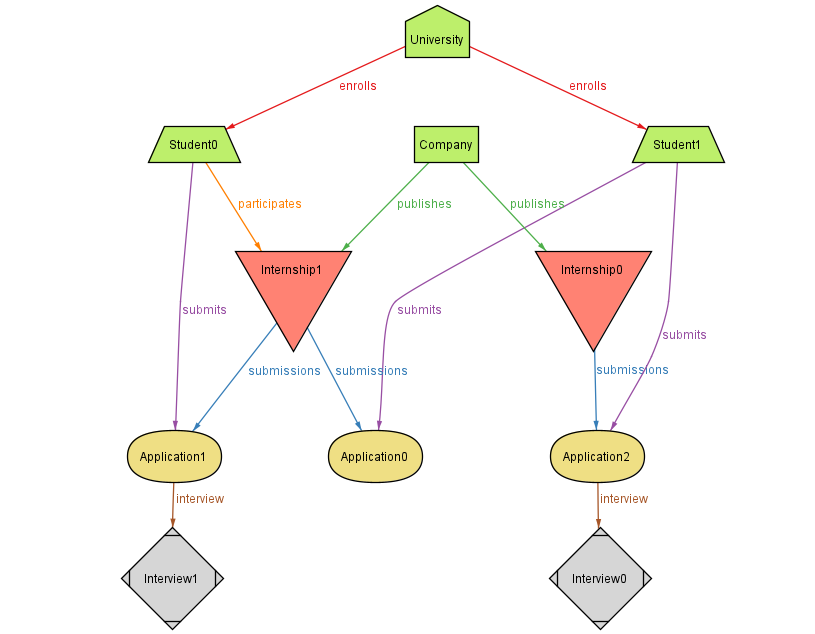
\includegraphics[width=0.75\textwidth]{Images/Alloy/example0.png}
    \caption{World generated by example 0}\label{fig:example0}
\end{figure}

\subsubsection{Scenario2 (Predicate 1)}
The following predicate describes a more structured model with 2 universities, 5 students, 3 internships, and 2 companies.
All students submit more than 1 application, all students participate in less internships than the number of applications they submitted,
at least 1 student participates in an internship, applications and feedbacks are more than 0, and the number of interviews is less than the 
number of applications.
\begin{lstlisting}
pred example1 {
    #University = 2
    #Student = 5
    #Internship = 3
    #Company = 2
    some s: Student | #s.submits > 1
    all s: Student | #s.participates < #s.submits
    some s: Student | #s.participates > 0
    #Application > 0
    #Feedback > 0
    #Interview < #Application
} 
run example1 for 9
\end{lstlisting}
\begin{figure}[H]
    \centering
    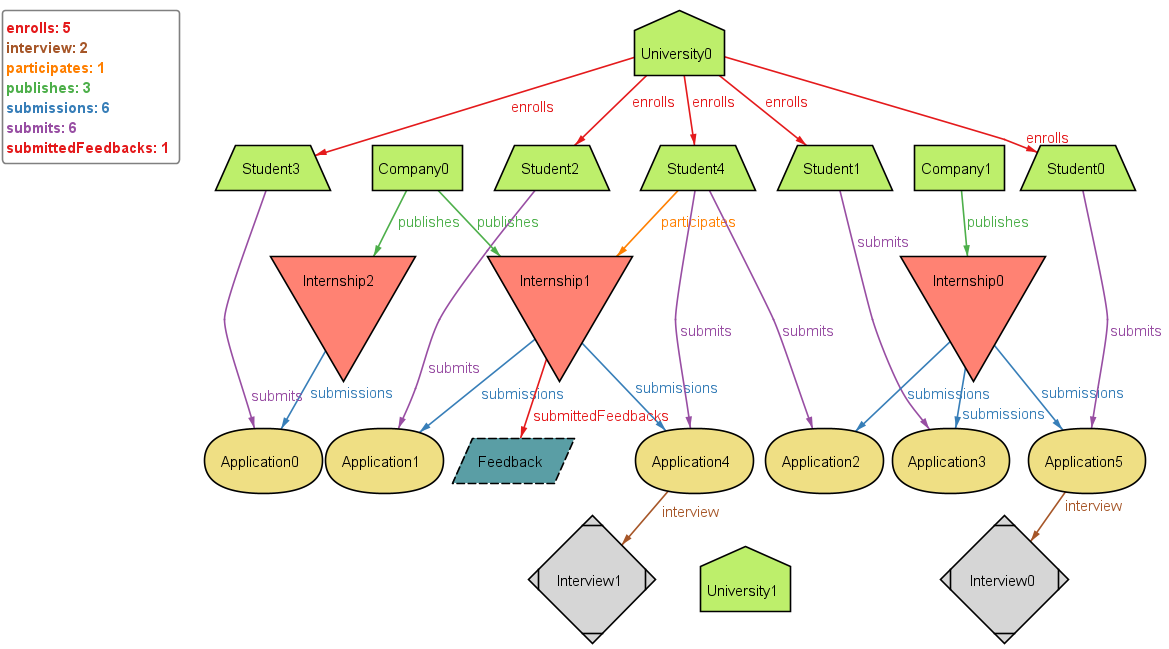
\includegraphics[width=1\textwidth]{Images/Alloy/example1.png}
    \caption{World generated by example 1}\label{fig:example1}
\end{figure}

\subsubsection{Scenario3 (Predicate 2)}
The following predicate describes a more complex model with 2 universities, 5 students, 5 internships, and 2 companies.
All universities have less than 3 students enrolled, at least 1 student submits more than 1 application, 
at least 1 student participates in an internship, at least 1 internship has no submissions,
all internships have less than 3 submitted feedbacks, and the number of submissions is greater than the 
number of students participating. Each company has less than 3 internships published.
\begin{lstlisting}
pred example2 {
    #University = 2     #Student = 5      #Internship = 5   #Company = 2
    #Application > 0    #Feedback > 0     #Interview < #Application
    all u: University | #u.enrolls <= 3
    all u: University | (some s: Student | s in u.enrolls and #s.submits > 0 and #s.participates > 0)
    some s: Student | #s.submits > 1
    all s: Student | #s.submits < 3
    some s: Student | #s.participates > 0
    some s: Student | #s.participates > 1
    some i: Internship | #i.submissions = 0
    all i: Internship | #i.submittedFeedbacks < 3
    all c: Company | #c.publishes <= 3
}
run example2 for 13
\end{lstlisting}
\begin{figure}[H]
    \centering
    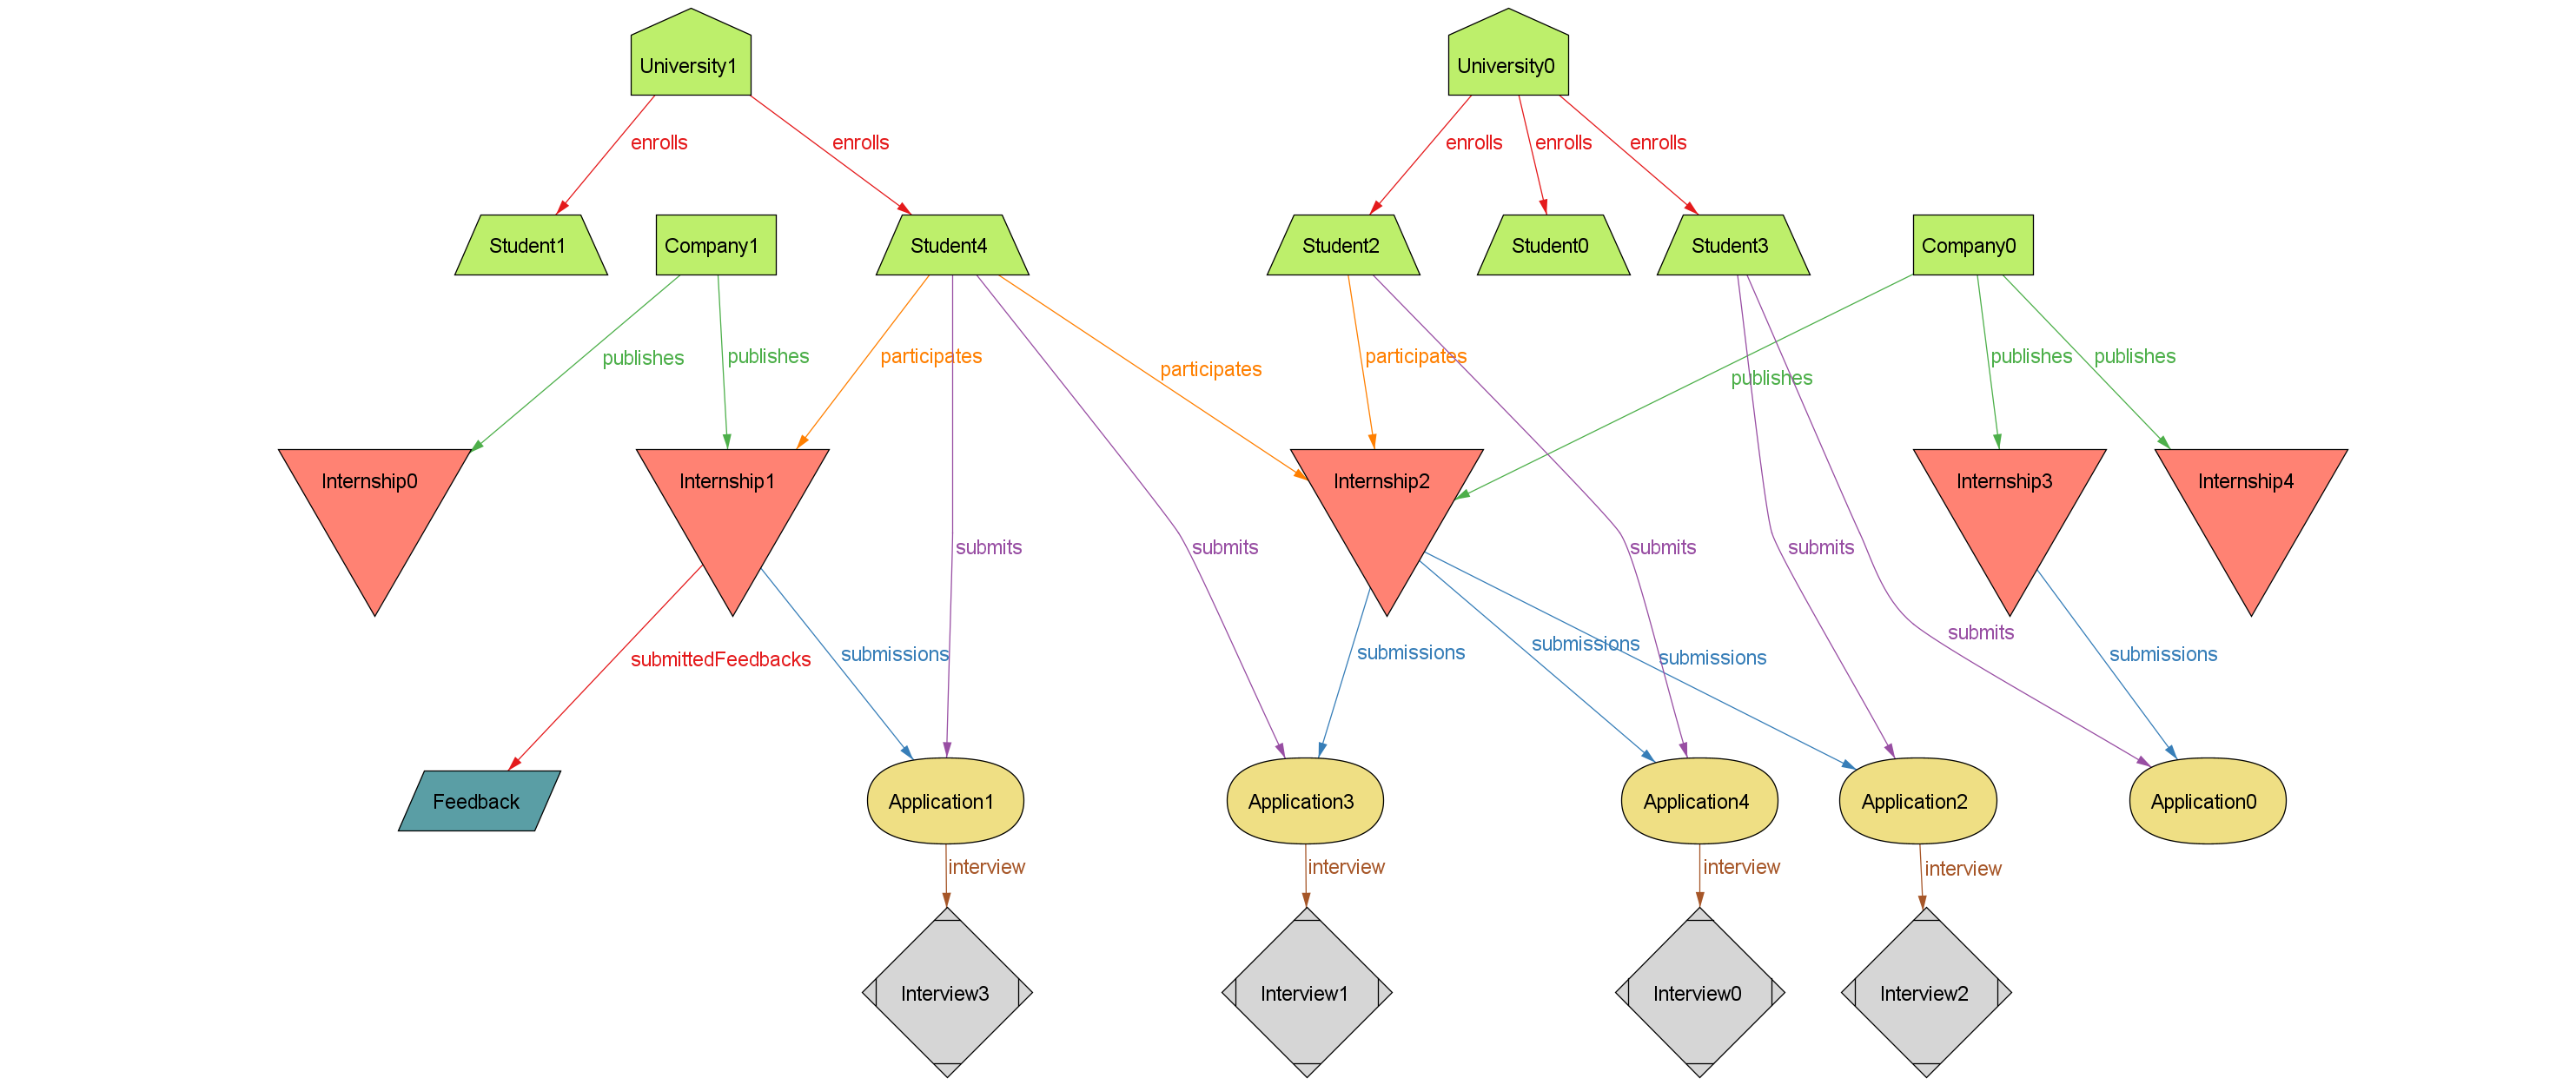
\includegraphics[width=1\textwidth]{Images/Alloy/example2.png}
    \caption{World generated by example 2}\label{fig:example2}
\end{figure}


\section{Dynamic part}
This model aims to describe the behavior of the system, focusing on the evolution of the system in time. In particular, we are going to
describe the evolution of the system when a student submits an application, when a company publishes an internship, when an interview is scheduled,
when a feedback is submitted, and when a student participates in an internship.

\subsubsection{Signatures}
The following signatures describe the main entities of the system:
\begin{lstlisting}
abstract sig User {}
sig Student extends User {
    var submits: set Application,
    var participates: set Internship
}{
    one u: University | this in u.enrolls
}
sig Company extends User {
    var publishes: set Internship
}
sig University extends User {
    var enrolls: set Student
}
var sig Internship {
    var submissions: set Application,
    var submittedFeedbacks: set Feedback,
    var internStatus: one InternshipStatus
}{
    one c: Company | this in c.publishes
}
var sig Application {
   var interview: lone Interview,
   var AppStatus: one ApplicationStatus
}{
    one s: Student | this in s.submits
    one i: Internship | this in i.submissions
}
var sig Feedback {} {
    one i: Internship | this in i.submittedFeedbacks
} 
var sig Interview {} {
    one a: Application | this in a.interview
}
//Model the status of an application
abstract sig ApplicationStatus{}
one sig SubmissionWaiting, SelectedToInterview, AcceptedToInternship, 
AcceptedOffer, RejectedOffer, Rejected extends ApplicationStatus{}
//Model the  status of internship:
abstract sig InternshipStatus{}
one sig InPublishing, InSelection, InProgress, Completed extends InternshipStatus{}
\end{lstlisting}

\subsubsection{Facts}
The following facts describe the constraints between the entities, relationships, and evolution of the system:
\begin{lstlisting}
//Facts used before in Static model 
// Fact to ensure that a student cannot submit multiple applications for the same internship
fact noRepeatedApplicationsForSameInternship{
   always (all s: Student, i: Internship | no disj a1,a2: s.submits | (a1 in i.submissions and a2 in i.submissions) )
}
// Fact to ensure that a feedback is submitted only if at least a student has participated in the internship
fact feedbackOnlyIfStudentInInternship{
    always( all f: Feedback, i: Internship | f in i.submittedFeedbacks 
     implies (some s: Student | i in s.participates and 
        (some a: Application | a in s.submits and a in i.submissions))
    )
}
// Fact to ensure that all internships where a student has participated have an interview scheduled for the application
fact allStudentInternshipsHaveInterviewInApplication{
    always( all s: Student, i: Internship | i in s.participates implies 
        (some a: Application | a in s.submits and a in i.submissions and
        (some intv: Interview | intv in a.interview))
    )
}

//Facts for the dynamic model
// Application can only be in one status at a time
fact ApplicationStatusCanOnlyHaveOnePhaseAtATime{
    always all a: Application | (one a.AppStatus and
    (a.AppStatus = SubmissionWaiting or 
    a.AppStatus = SelectedToInterview or 
    a.AppStatus = AcceptedToInternship or 
    a.AppStatus = AcceptedOffer or 
    a.AppStatus = Rejected or 
    a.AppStatus = RejectedOffer))
}
//Internship can only be in one possible status at a time
fact InternshipStatusCanOnlyHaveOnePhaseAtATime {
    always all i: Internship | one i.internStatus and 
    (i.internStatus = InPublishing or
    i.internStatus = InSelection or
    i.internStatus = InProgress or
    i.internStatus = Completed)
}
// Fact to describe the possible statuses of the applications in each state of the internship
fact allowedAppStatusInEachInternshipStatus {
    always( all i: Internship | 
        (i.internStatus = InPublishing implies 
            (all a: i.submissions | a.AppStatus = SubmissionWaiting)) and 
        (i.internStatus = InSelection implies 
            (all a: i.submissions | a.AppStatus = SelectedToInterview or a.AppStatus = Rejected or a.AppStatus = AcceptedToInternship)) and
        (i.internStatus = InProgress implies 
            (all a: i.submissions | a.AppStatus = AcceptedOffer or a.AppStatus = Rejected or a.AppStatus = RejectedOffer) and (some a: i.submissions | a.AppStatus = AcceptedOffer)) and 
        (i.internStatus = Completed implies  
            (all a: i.submissions | a.AppStatus = AcceptedOffer or a.AppStatus = Rejected or a.AppStatus = RejectedOffer) and (some a: i.submissions | a.AppStatus = AcceptedOffer))
    )
}
// Variation of Interview in every state of the application
fact InterviewInEveryStateOfApplication{
    always all a: Application | 
    (a.AppStatus = SubmissionWaiting implies a.interview = none) and
    (a.AppStatus = SelectedToInterview implies a.interview != none) and
    (a.AppStatus = AcceptedToInternship implies a.interview != none) and
    (a.AppStatus = AcceptedOffer implies a.interview != none) and
    (a.AppStatus = RejectedOffer implies a.interview != none) and
    ((a.AppStatus = Rejected and a.interview != none) implies after always a.interview != none) and
    ((a.AppStatus = Rejected and a.interview = none) implies after always a.interview = none)
}
// When an interview is scheduled for an application, it should never be removed
fact InInterviewCanNotBeRemoved{
    always all a: Application | a.interview != none implies (a.interview' = a.interview)
}
// Student cannot change the university that he is enrolled in
fact studentUniversityInvariant{
    always (all s: Student, u:University | s in u.enrolls implies (after always s in u.enrolls))
}
// Internship cannot change the company that published it
fact internshipCompanyInvariant{
    always (all i: Internship, c:Company | i in c.publishes implies (after always i in c.publishes))
}
// Application cannot change the student that submitted it
fact applicationStudentInvariant{
    always (all a: Application, s:Student | a in s.submits implies (after always a in s.submits))
}
// Student cannot remove the internship that he has participated in
fact studentInternshipInvariant{
    always (all s: Student, i:Internship | i in s.participates implies (after always i in s.participates))
}
// Application cannot change the internship that it is submitted for
fact applicationInternshipInvariant{
    always (all a: Application, i:Internship | a in i.submissions implies (after always a in i.submissions))
}
//Feedback cannot change the internship that it is submitted for
fact feedbackInternshipInvariant{
    always (all f: Feedback, i:Internship | f in i.submittedFeedbacks implies (after always f in i.submittedFeedbacks))
}
// Fact to describe the possible status evolution of the internship
fact internshipStatusAllowedEvolution {
    always( no i: Internship | 
        i.internStatus = InPublishing and (i.internStatus' = InProgress or i.internStatus' = Completed)
        or
        i.internStatus = InSelection and (i.internStatus' = InPublishing or i.internStatus' = Completed)
        or
        i.internStatus = InProgress and (i.internStatus' = InSelection or i.internStatus' = InPublishing)
        or
        i.internStatus = Completed and (i.internStatus' = InSelection or i.internStatus' = InProgress or i.internStatus' = InPublishing)
    )
}
// Fact to describe the possible status evolution of the application
fact allowedAppEvol {
    always (no a: Application | 
        a.AppStatus = SubmissionWaiting and (a.AppStatus' = AcceptedOffer or a.AppStatus' = RejectedOffer or a.AppStatus' = AcceptedToInternship)
        or
        a.AppStatus = SelectedToInterview and (a.AppStatus' = AcceptedOffer or a.AppStatus' = RejectedOffer or a.AppStatus' = SubmissionWaiting)
        or
        a.AppStatus = AcceptedToInternship and (a.AppStatus' = Rejected or a.AppStatus' = SelectedToInterview or a.AppStatus' = SubmissionWaiting)
        or
        a.AppStatus = AcceptedOffer and (a.AppStatus' = Rejected or a.AppStatus' = RejectedOffer or a.AppStatus' = AcceptedToInternship or a.AppStatus' = SelectedToInterview or a.AppStatus' = SubmissionWaiting)
        or
        a.AppStatus = RejectedOffer and (a.AppStatus' = Rejected or a.AppStatus' = AcceptedOffer or a.AppStatus' = AcceptedToInternship or a.AppStatus' = SelectedToInterview or a.AppStatus' = SubmissionWaiting)
        or
        a.AppStatus = Rejected and (a.AppStatus' = AcceptedOffer or a.AppStatus' = RejectedOffer or a.AppStatus' = AcceptedToInternship or a.AppStatus' = SelectedToInterview or a.AppStatus' = SubmissionWaiting)
    )
}
// An internship in publishing or selection cannot have students participating in it and feedbacks submitted
fact NoStudentsOrFeedbacksInInternshipInPublishingOrSelection{
    always all i: Internship | (i.internStatus = InPublishing or i.internStatus = InSelection) implies
    (no s: Student | i in s.participates) and (no f: Feedback | f in i.submittedFeedbacks)
}
// When internship is in publishing status, no applications submitted should have an interview scheduled
fact noInterviewsWhileInternshipInPublishing {
    always all i: Internship | i.internStatus = InPublishing implies (no a: i.submissions | a.interview != none)
}
// An application can be submitted to the internship only if the internship is in publishing status
fact SubmissionsMutableOnlyInPublishing {
    always all i: Internship | (i.internStatus != InPublishing or i.internStatus' != InPublishing) implies (i.submissions' = i.submissions)
}
// An internship can be in selection status only if at least one application has been submitted
fact InternshipInSelectionOnlyIfApplicationSubmitted{
    always all i: Internship | i.internStatus = InSelection implies (some a: Application | a in i.submissions)
}
// All applications of an internship in selection move from state SelectedToInterview to AcceptedToInternship (or Rejected) at the same step
fact NoSimultaneousSelectedAndAccepted {
    always all i: Internship | (i.internStatus = InSelection and some a: i.submissions | a.AppStatus = AcceptedToInternship) implies (all a: i.submissions | a.AppStatus = AcceptedToInternship or a.AppStatus = Rejected)
}
// If a student participates to an internship, then that internship is in progress or completed
fact NoStudentParticipatesInInternshipIfNotInProgressOrCompleted{
    always all s: Student, i: Internship | i in s.participates implies (i.internStatus = InProgress or i.internStatus = Completed)
}
// An internship can be in progress or completed only if at least one student participates in it
fact InternshipInProgressOrCompletedOnlyIfStudentParticipates{
    always all i: Internship | (i.internStatus = InProgress or i.internStatus = Completed) implies (some s: Student | i in s.participates)
}
// When an internship is in progress status or completed status, all applications should be in the final status: accepted offer, rejected offer or rejected
fact InternshipInProgressOrCompletedApplicationsInFinalStatus{
    always all i: Internship | (i.internStatus = InProgress or i.internStatus = Completed) implies
    (all a: i.submissions | (a.AppStatus = AcceptedOffer or a.AppStatus = RejectedOffer or a.AppStatus = Rejected))
}
// Every Student can only do one internship at a time
fact StudentCanDoOneInternshipsAtATime{
    always all s: Student | let concurrentParticipations = #(s.participates & {i: s.participates | i.internStatus = InProgress}) |
    concurrentParticipations <= 1
}
// Student application number should be more or equals to the number of internships they participated in
fact StudentApplicationsMoreThanParticipations{
    always all s: Student | #s.submits >= #s.participates 
}
// Student should have the offer accepted equal or less than the number of applications submitted and equal to the number of participations
fact StudentOffersAccepted{
    always all s: Student | 
    let numOffersAccepted = #(s.submits & {a: s.submits | a.AppStatus = AcceptedOffer}) |
    let numApplications = #s.submits |
    let numParticipations = #s.participates |
    numOffersAccepted <= numApplications and numOffersAccepted = numParticipations
}
// Student has participated if and only if he accepted the application related to the internship
fact StudentParticipatesInInternship{
    always all s: Student, i: Internship | i in s.participates implies
    (some a: Application | a in s.submits and a in i.submissions and a.AppStatus = AcceptedOffer)
}
// When an internship is in progress or completed, no more interviews should be scheduled
fact noChangeInInterviewsWhenInternshipInProgressOrCompleted{
    always all i: Internship | (i.internStatus = InProgress or i.internStatus = Completed) implies
    i.submissions.interview' = i.submissions.interview
}
// Once Internship is completed, no more feedbacks can be submitted
fact InternshipCompletedNoMoreFeedbacks{
    always all i: Internship | i.internStatus' = Completed implies (i.submittedFeedbacks' = i.submittedFeedbacks)
}
// Once Internship is in progress, feedbacks can be submitted
fact InProgressForFeedbacks{
    always all i: Internship | (#i.submittedFeedbacks' > #i.submittedFeedbacks) implies i.internStatus = InProgress
}
// Once Internship is completed, there should be at least 2 feedbacks
fact AtLeast2FeedbackIfCompleted{
    always all i: Internship | i.internStatus' = Completed implies (#i.submittedFeedbacks > 1)
}

//Initialization
// Forcing the initial state of the system
fact init {
    #University = 1
    #Company = 1
    #Student = 4
    #Internship = 1
    all i: Internship | i.internStatus = InPublishing
}
\end{lstlisting}

\subsubsection{Predicates and Scenario}
In this section we are going to describe the evolution of the system in time, 
focusing on the main actions that can be performed by the users of the system.

\begin{lstlisting}
// Predicates to model the creation of an internship
pred internshipCreation {
    eventually (#Internship = 2 and all i: Internship | i.internStatus = InPublishing and after always #Internship = 2) and 
	always (all a: Application, i: Internship | (a in i.submissions and a.AppStatus = SubmissionWaiting) implies before i.internStatus = InPublishing)
}
// Predicates to model the submission of an application
pred applicationSubmission {
    eventually (some a: Application, s: Student, i: Internship | a in s.submits and a in i.submissions and a.AppStatus = SubmissionWaiting) and eventually #Application > 2
}
// Predicates to model the rejection of an application
pred applicationRejection {
    eventually (some s: Student, i: Internship, a: Application  | a in s.submits and a in i.submissions and a.AppStatus = Rejected)
}
// Predicates to model the selection of an application
pred applicationSelection {
    eventually (some s: Student, i: Internship, a: Application  | a in s.submits and a in i.submissions and a.AppStatus = SelectedToInterview)
}
// Predicates to model the acceptance of an application
pred applicationAcceptance {
    eventually (some s: Student, i: Internship, a: Application  | a in s.submits and a in i.submissions and a.AppStatus = AcceptedToInternship)
}
// Predicates to model the acceptance of an internship
pred internshipAcceptance {
    eventually (some s: Student, i: Internship, a: Application  | a in s.submits and a in i.submissions and a.AppStatus = AcceptedOffer)
}
// Predicates to model the rejection of an internship
pred internshipRejection {
    eventually (some s: Student, i: Internship, a: Application  | a in s.submits and a in i.submissions and a.AppStatus = RejectedOffer)
}
// Predicates to model the submission of a feedback
pred feedbackSubmission {
    eventually (some f: Feedback, i: Internship | f in i.submittedFeedbacks)
}
// Predicates to model the completion of all internships
pred allInternshipCompleted {
    eventually (all i: Internship | i.internStatus = Completed)
}
// RUN THE SYSTEM
run { internshipCreation;applicationSubmission;applicationRejection;
    applicationSelection;applicationAcceptance;internshipAcceptance;
    internshipRejection;feedbackSubmission;allInternshipCompleted 
} for 7
\end{lstlisting}

\begin{figure}
    \centering
    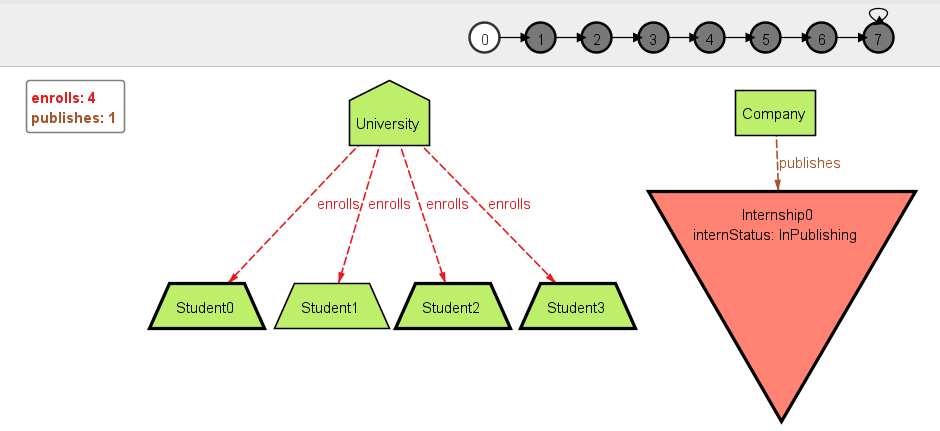
\includegraphics[width=1\textwidth]{Images/Alloy/dyn1.png}\label{fig:dyn1}
\end{figure}
\begin{figure}
    \centering
    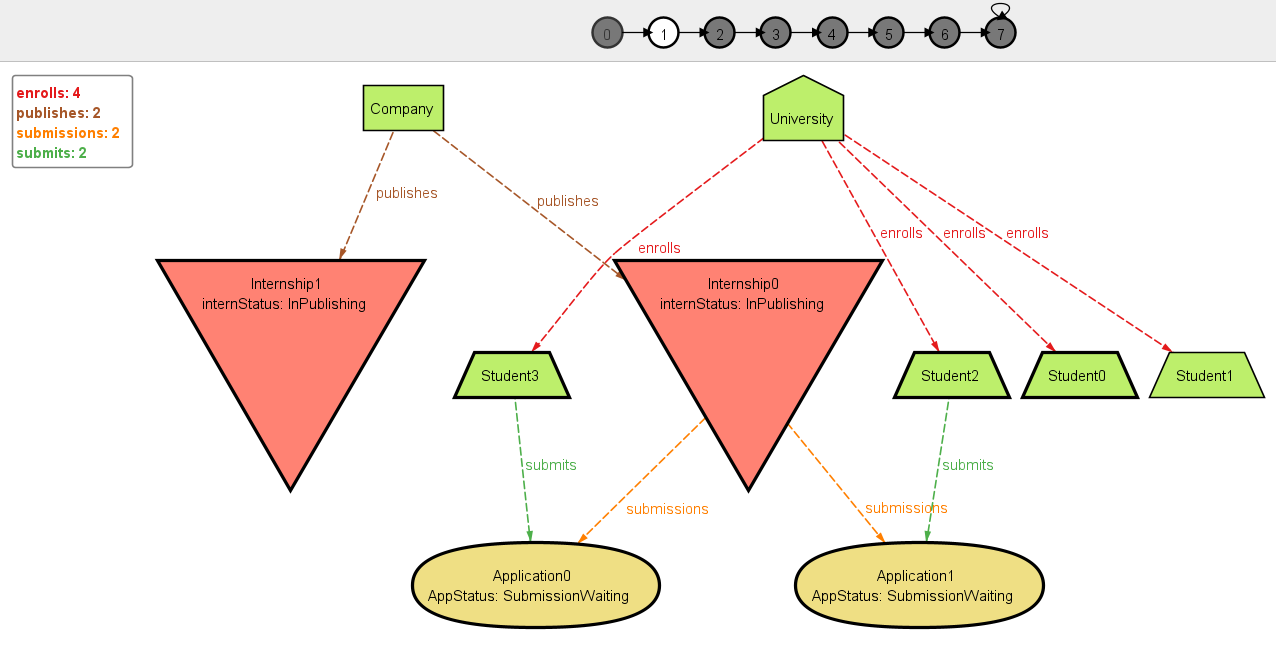
\includegraphics[width=1\textwidth]{Images/Alloy/dyn2.png}\label{fig:dyn2}
\end{figure}
\begin{figure}
    \centering
    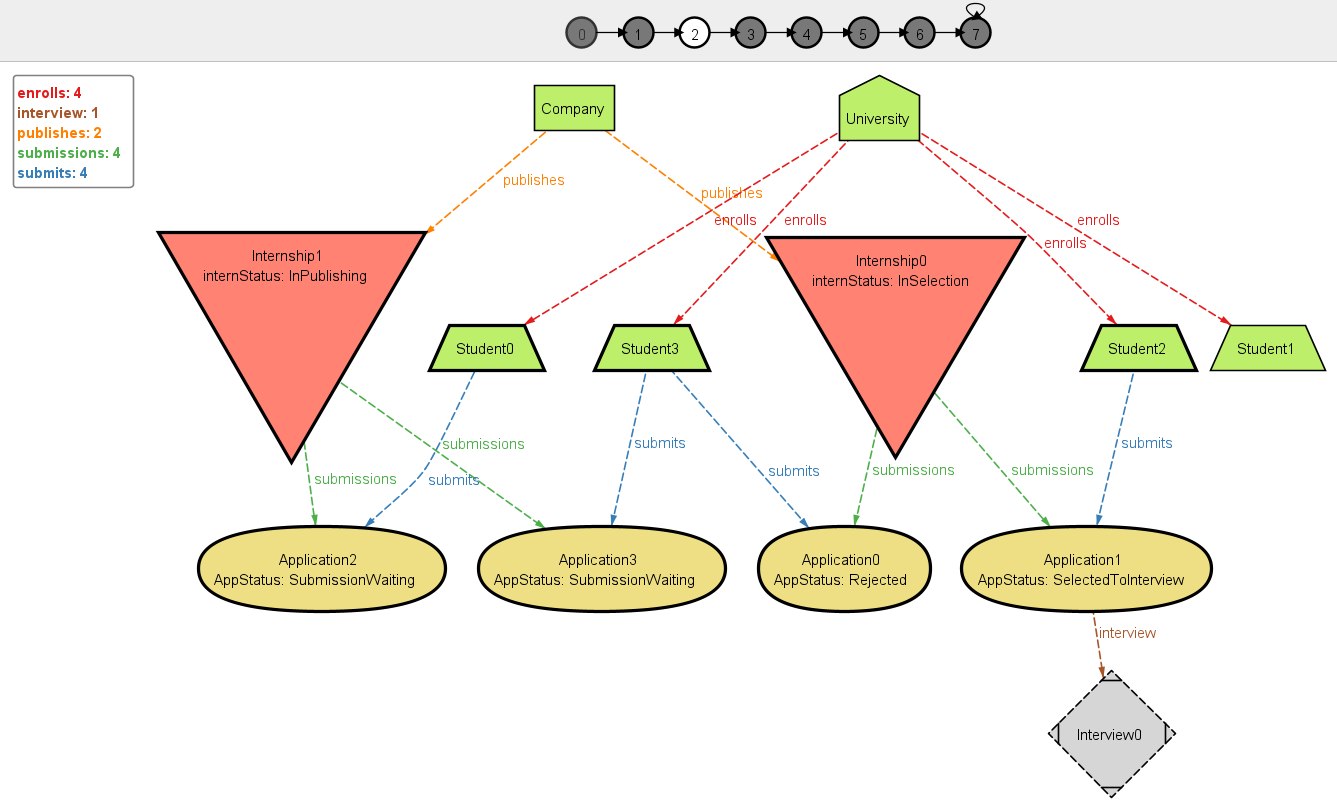
\includegraphics[width=1\textwidth]{Images/Alloy/dyn3.png}\label{fig:dyn3}
\end{figure}
\begin{figure}
    \centering
    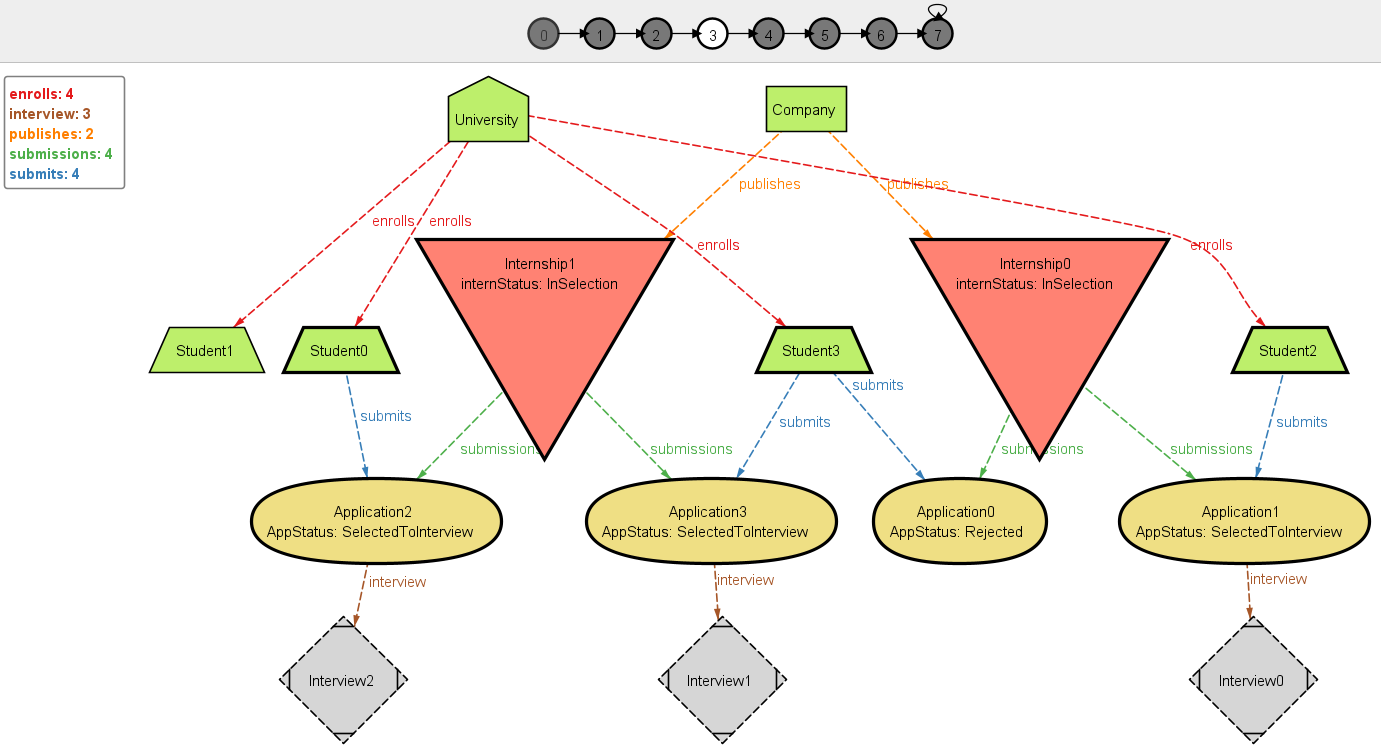
\includegraphics[width=1\textwidth]{Images/Alloy/dyn4.png}\label{fig:dyn4}
\end{figure}
\begin{figure}
    \centering
    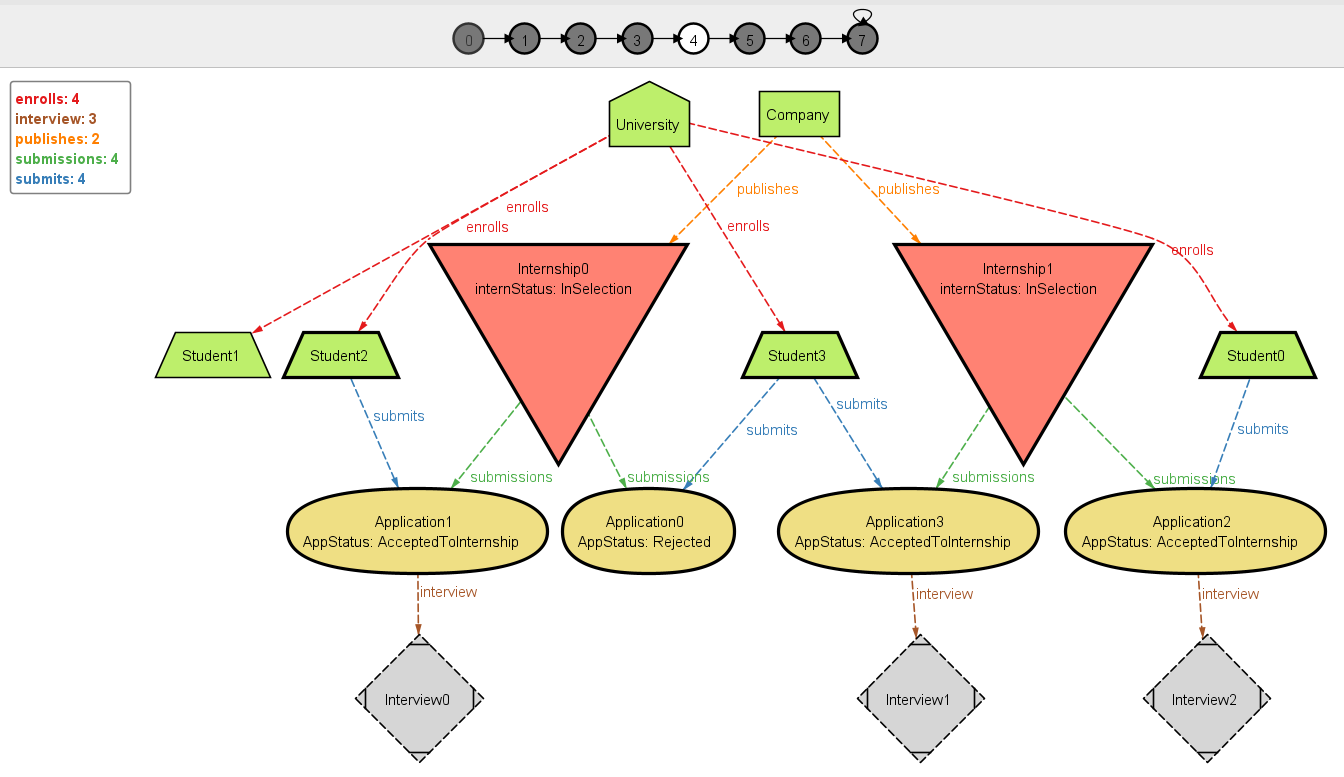
\includegraphics[width=1\textwidth]{Images/Alloy/dyn5.png}\label{fig:dyn5}
\end{figure}
\begin{figure}
    \centering
    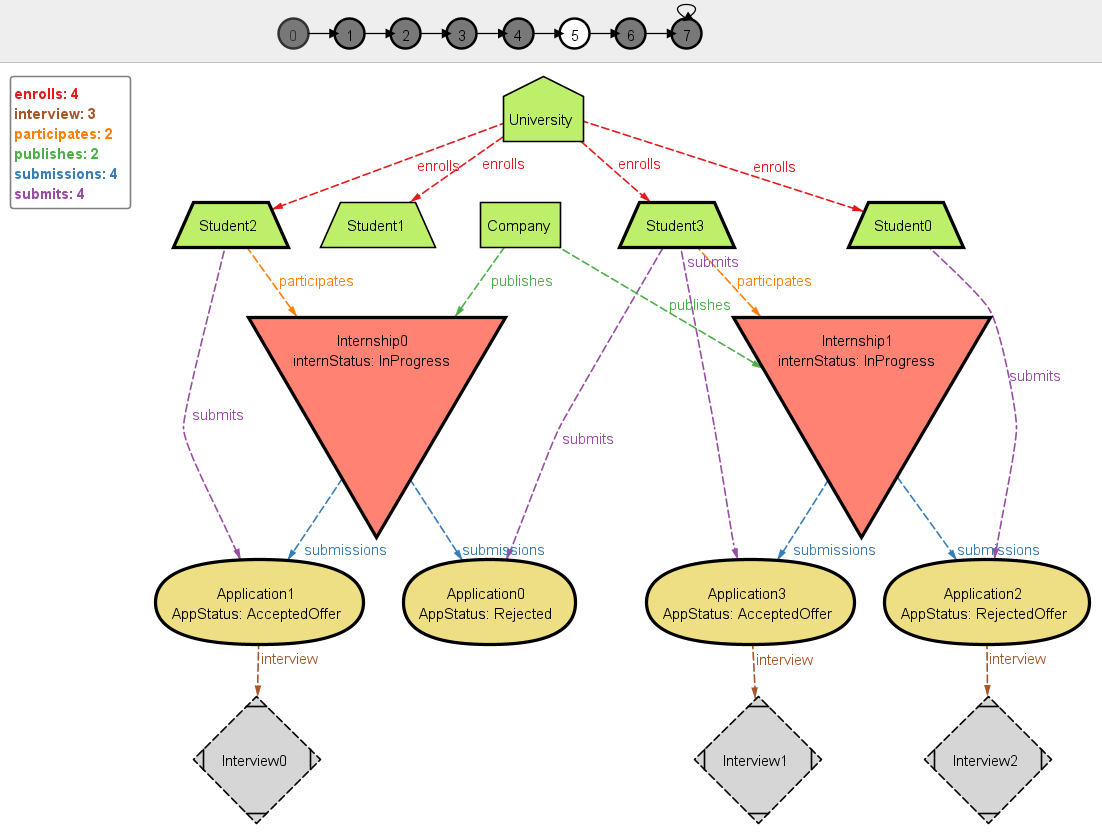
\includegraphics[width=1\textwidth]{Images/Alloy/dyn6.png}\label{fig:dyn6}
\end{figure}
\begin{figure}
    \centering
    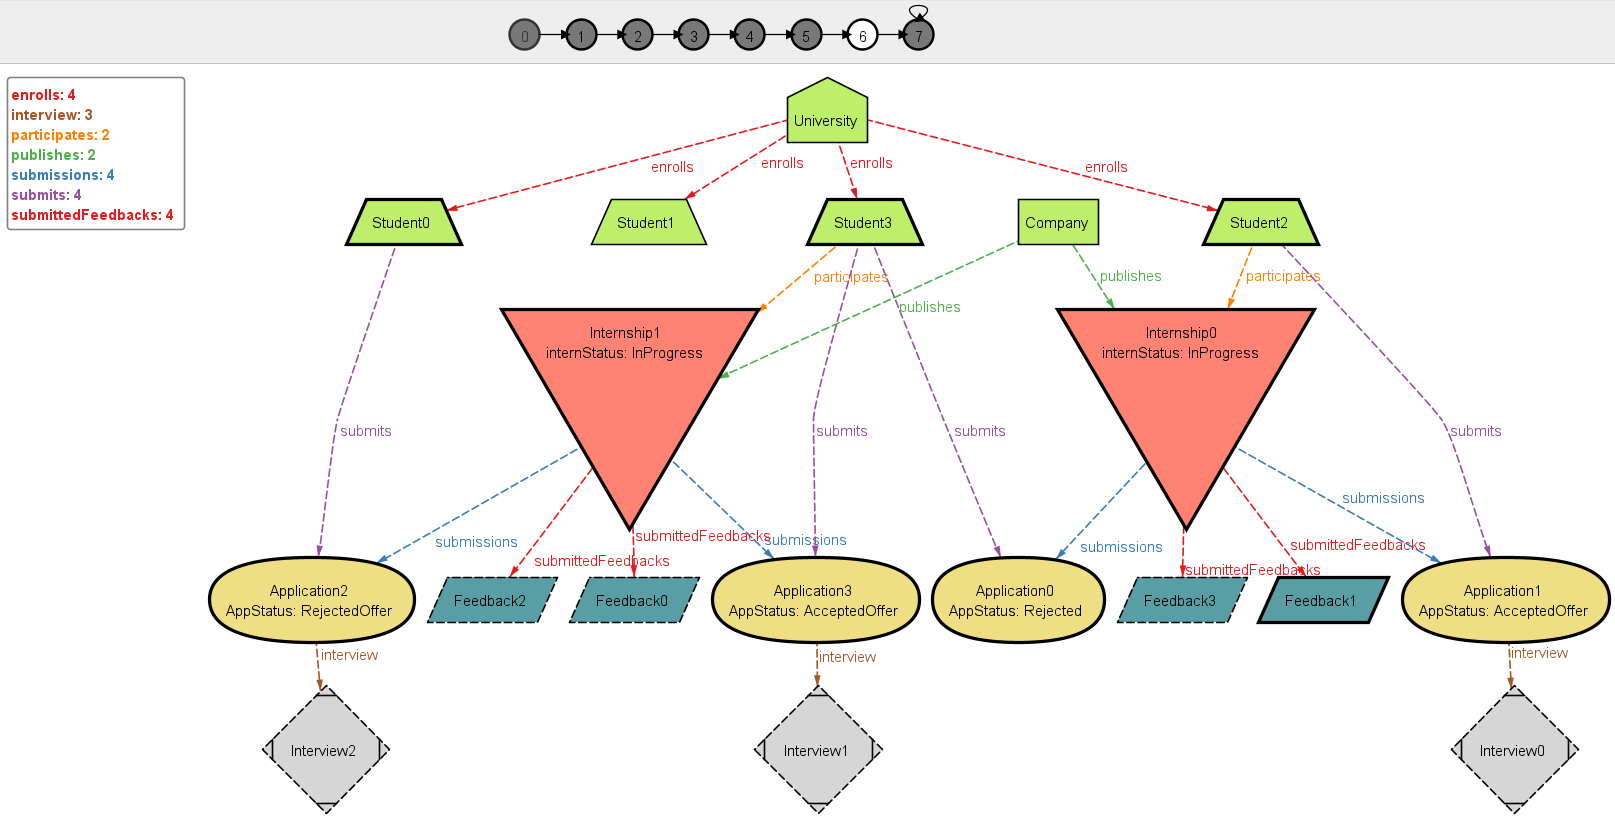
\includegraphics[width=1\textwidth]{Images/Alloy/dyn7.png}\label{fig:dyn7}
\end{figure}
\begin{figure}
    \centering
    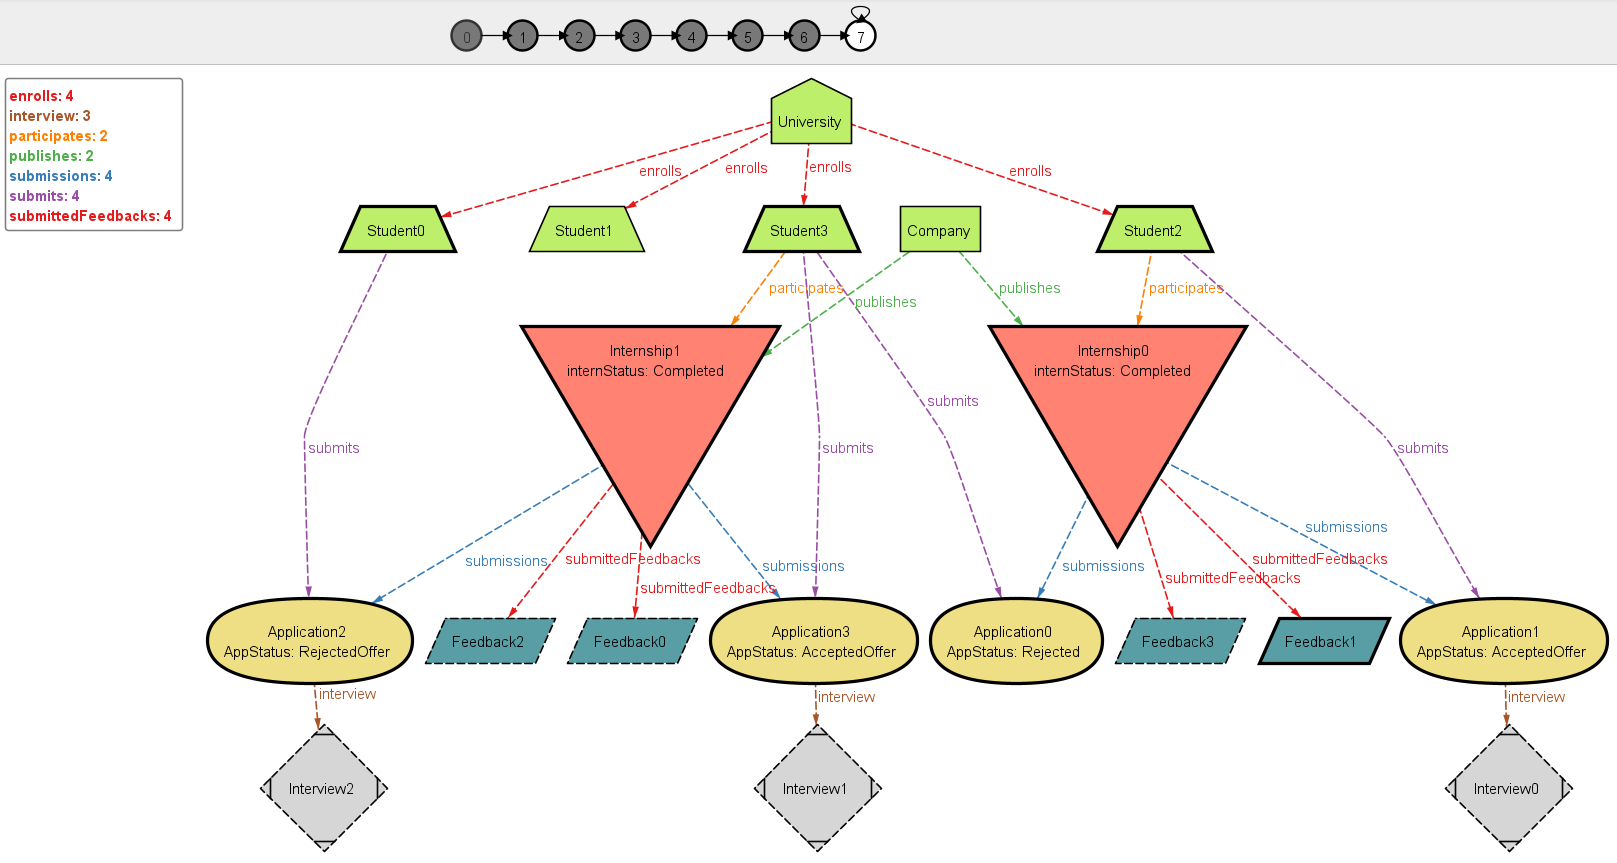
\includegraphics[width=1\textwidth]{Images/Alloy/dyn8.png}\label{fig:dyn8}
\end{figure}

\clearpage
{\color{Blue}{\section{Effort Spent}}}
\label{sect:effort}
In following table we provide the tracking of the effort spent by each group member in the development of this document.
\begin{table}[H]
    \centering
    \begin{tabular}{|c|c|c|}
    \hline
    \rowcolor{bluepoli!40}
    \textbf{Section} & \textbf{Jie Chen} & \textbf{Riccardo Bonfanti} \T\B \\
    \hline
     \textbf{1 – Introduction}                  & 0 hours & 1.5 hours \T\B \\
     \textbf{2 – Architectural Design}           & 0 hours & 27 hours \T\B\\
     \textbf{3 – User Interface Design}         & 0 hours & 0 hours \T\B\\
     \textbf{4 – Requirements Traceability}   & 0 hours & 2 hours  \T\B \\
     \textbf{5 – Implementation, Integration, and Test Plan}   & 0 hours & 0 hours  \T\B \\
     \hline
     \textbf{Total}                             & 0 hours & 31.5 hours \T\B \\

    \hline
    \end{tabular}
    \\[10pt]
    \caption{Effort spent for each section}\label{table:effort}
\end{table}

\clearpage
\addcontentsline{toc}{section}{References}
\bibliographystyle{plain}
\bibliography{main}

\end{document}